\chapter{Experimental Setup and Results}\label{ch:4}
This chapter presents the empirical results that validate the decoupled, deep metric learning framework proposed in Chapter~\ref{ch:3}. The central objective is to exhaustively assess the performance of each component of the pipeline---from the choice of embedding model and the impact of fine-tuning to the effects of dimensionality reduction and the selection of a downstream classifier---to identify the optimal configuration for both classification accuracy and computational efficiency.

The analysis is structured to first establish the validity of the core feature engineering approach before proceeding through the primary evaluation sequence. The chapter begins by presenting an ablation study to validate the efficacy of the novel composite distance vector (\(\Delta_c\)), the cornerstone of the feature representation. With the feature vector's design validated, the investigation then establishes a baseline by assessing off-the-shelf models, quantifies the performance gains achieved through fine-tuning, and analyzes the trade-offs between accuracy and efficiency. The chapter culminates in a definitive comparative analysis on the held-out test data, synthesizing all prior findings to identify the single best-performing pipeline configuration. We begin by outlining the experimental setup that forms the foundation for all subsequent results.

\section{Experimental Environment \& Datasets}\label{ch:4.1}

\subsection{Computational Environment}\label{ch:4.1.1}
The research presented in this thesis was conducted using a hybrid computational environment, leveraging both cloud-based services for initial language model evaluations and a powerful on-premise high-performance computing (HPC) cluster for the primary, computationally intensive experiments. The initial direct classification tasks were performed using Google's Gemini v1.0, a proprietary cloud-based Large Language Model. All subsequent stages, including model fine-tuning and downstream classifier evaluations, were executed on San Francisco State University's ``POLARIS'' High Performance Compute Cluster. The POLARIS cluster runs on Rocky Linux 8.9 with the Slurm Workload Manager. GPU-intensive deep learning tasks were performed on a node equipped with four NVIDIA A100 GPUs, while extensive hyperparameter grid searches for traditional machine learning classifiers were run on a CPU cluster with AMD EPYC 9534 CPUs. The entire experimental pipeline was implemented in Python, with the core deep learning components built using PyTorch and the Hugging Face ecosystem and the classical machine learning experiments conducted using \verb|scikit-learn| and \verb|XGBoost|.

\subsection{Datasets}\label{ch:4.1.2}
As detailed in Chapter~\ref{ch:3}, this research utilized two distinct datasets at different stages of the evaluation. A smaller \textbf{Initial Dataset}, manually curated from the ASSIST repository, was used for prototyping and the preliminary screening of models and classifiers. The definitive experiments were conducted on the larger \textbf{PPM Corpus}, provided by the Program Pathways Mapper (PPM). This corpus was used for the definitive fine-tuning and final pipeline evaluation, with its held-out test set reserved for an unbiased assessment of the optimized pipelines to ensure methodological rigor. Table~\ref{tbl:datasets} provides a summary of the key characteristics of both datasets.

\begin{table}[tb]
    \captionsetup{skip=5pt}
    \centering
    \caption{Summary of Datasets Used in Evaluation}
    \label{tbl:datasets}
    \resizebox{\columnwidth}{!}{
        \begin{tabular}{p{0.2\textwidth} p{0.4\textwidth} p{0.4\textwidth}}
            \toprule
            \textbf{Characteristic} & \textbf{Initial Dataset}                                      
            & \textbf{PPM Corpus}                                  \\
            \midrule
            \textbf{Source}         & Manually curated via ASSIST                   
            & Program Pathways Mapper (PPM)                        \\
            \addlinespace
            \textbf{Purpose}        & Preliminary screening, prototyping, and initial classifier evaluation & Definitive fine-tuning and final pipeline evaluation \\
            \addlinespace
            \textbf{Ground Truth}   & Established articulation agreements                                   & Course Identification Number (C-ID)                  \\
            \addlinespace
            \textbf{Final Size}     & 400 course pairs (for evaluation set)                                 & 2,157 courses (across 157 classes)                   \\
            \addlinespace
            \textbf{Partitioning}   & Stratified random sample                                              & Stratified 50/50 train/test split                    \\
            \bottomrule
        \end{tabular}
    }
\end{table}

\subsection{Evaluation Metrics}\label{ch:4.1.3}
To facilitate a multi-faceted analysis, a standard suite of metrics was used to assess both classification efficacy and computational efficiency. The core assessment of classification performance was measured using the \(F_1\)-Score, the harmonic mean of Precision and Recall. This metric was chosen because it provides a single, robust value that balances the trade-off between avoiding false equivalencies (precision) and identifying all true ones (recall), making it ideal for this task. For assessing practical viability, both Training Time and Inference Time were captured. Inference time is considered the more meaninful efficiency metric for this research, as it directly impacts the system's real-world responsiveness and scalability in a production environment.

\section{Baseline Performance: Direct LLM Classification}\label{ch:4.2}
The initial phase of this research sought to establish a performance baseline by evaluating the feasibility of using a Large Language Model for end-to-end course equivalency classification, a methodology detailed in Section~\ref{ch:3.1}. The experiments were conducted on the Initial Dataset, leveraging Google's Gemini Pro v1.0 as the reasoning engine. The results were encouraging, with the model achieving a peak accuracy of 90.5\% when using full, unprocessed raw text as input. This approach consistently yielded superior results compared to using only extracted structured topics. This performance gap is likely attributable to the challenges inherent in the data extraction step itself, which proved to be difficult and highly sensitive to prompt wording---a finding that aligns with previous studies on prompt engineering~\cite{Sclar2023QuantifyingLM,Errica2024WhatDI,Chen2024LLMAA,Cheung2024ARC,Gerych2024WhoKT}.

An analysis of the confusion matrices, presented in Figure~\ref{fig:cm}, reveals a consistent and telling behavioral pattern: the model exhibits a strong conservative bias. Across all scenarios, it was far more likely to misclassify a truly equivalent course pair as not equivalent (a false negative) than it was to incorrectly approve a non-equivalent pair (a false positive), suggesting the LLM operates with a high internal threshold for declaring equivalency. Furthermore, the experiments that introduced ``unsure'' and ``insufficient data'' categories demonstrated the model's ability to effectively isolate ambiguous cases that would require manual review. A comprehensive summary of the performance metrics is provided in Table~\ref{tbl:llm_results_summary}, and a comparative benchmark against other prominent LLMs is shown in Table~\ref{tbl:cls}.
\begin{figure}[tb]
    \captionsetup{skip=5pt}
    \centering
    \begin{subfigure}[b]{0.497\textwidth}
        \centering
        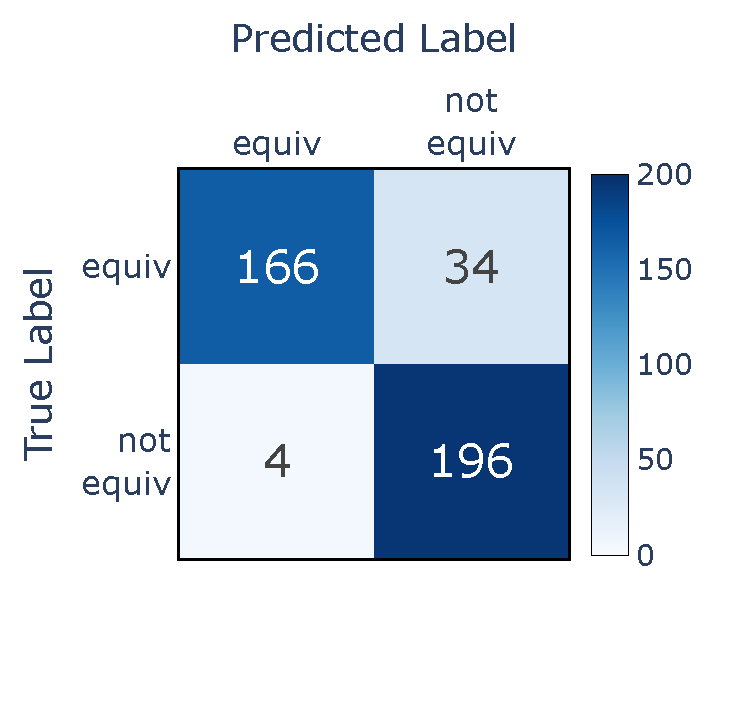
\includegraphics[scale=0.395,trim={3mm 20mm 7mm 0},clip]{LLMeval_binary_raw_text_cm.pdf}
        \caption{Binary Raw Text}
        \label{fig:sub_brt}
    \end{subfigure}
    \hfill
    \begin{subfigure}[b]{0.497\textwidth}
        \centering
        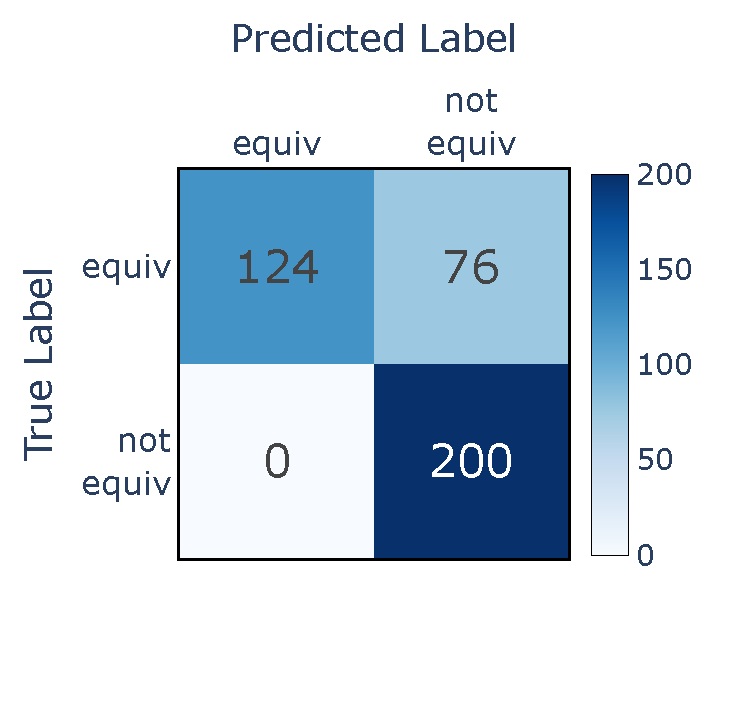
\includegraphics[scale=0.42,trim={3mm 20mm 7mm 0},clip]{LLMeval_binary_topics_cm.pdf}
        \caption{Binary Topics}
        \label{fig:sub_brt}
    \end{subfigure}

    \vspace{2mm}

    \begin{subfigure}[b]{0.497\textwidth}
        \centering
        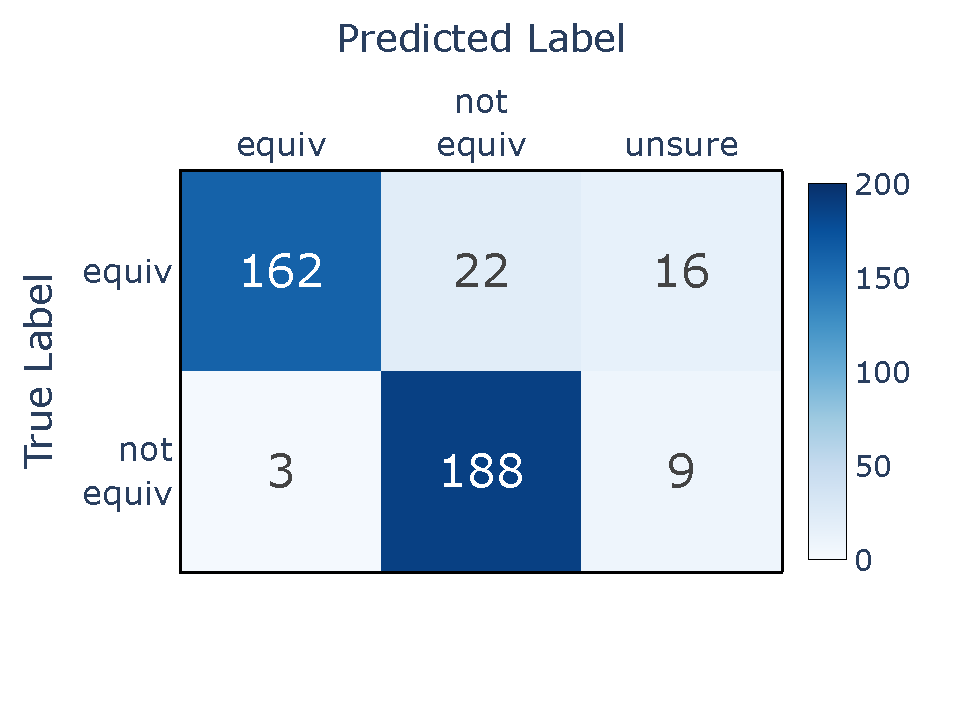
\includegraphics[scale=0.42,trim={3mm 20mm 7mm 0},clip]{LLMeval_3way_raw_text_cm.pdf}
        \caption{3-way Raw Text}
        \label{fig:sub_brt}
    \end{subfigure}
    \hfill
    \begin{subfigure}[b]{0.497\textwidth}
        \centering
        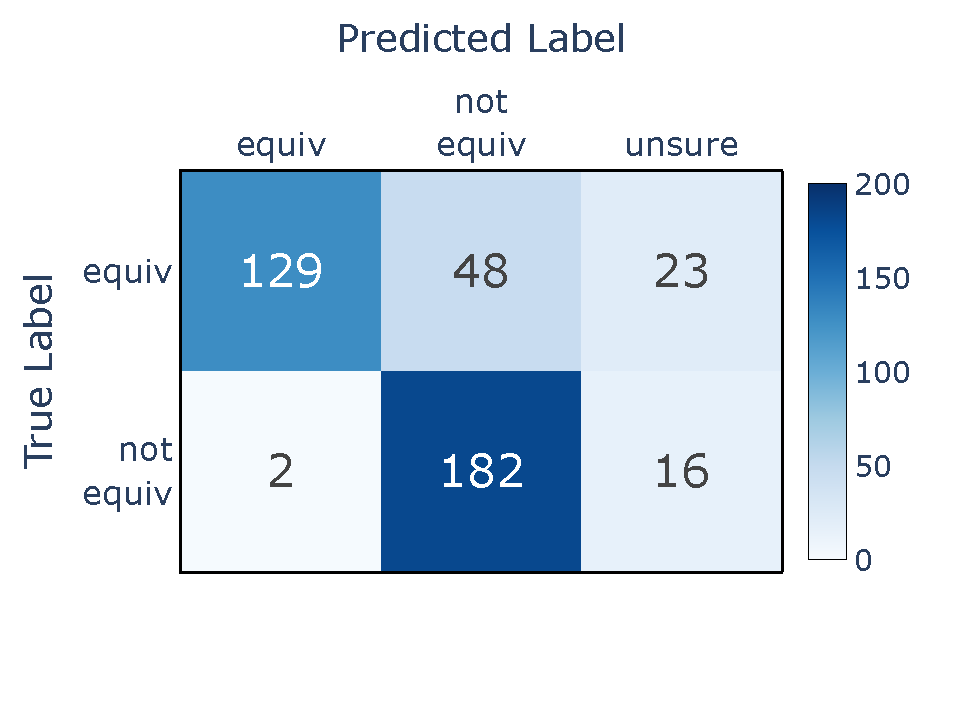
\includegraphics[scale=0.42,trim={3mm 20mm 7mm 0},clip]{LLMeval_3way_topics_cm.pdf}
        \caption{3-way Topics}
        \label{fig:sub_brt}
    \end{subfigure}

    \vspace{2mm}

    \begin{subfigure}[b]{0.497\textwidth}
        \centering
        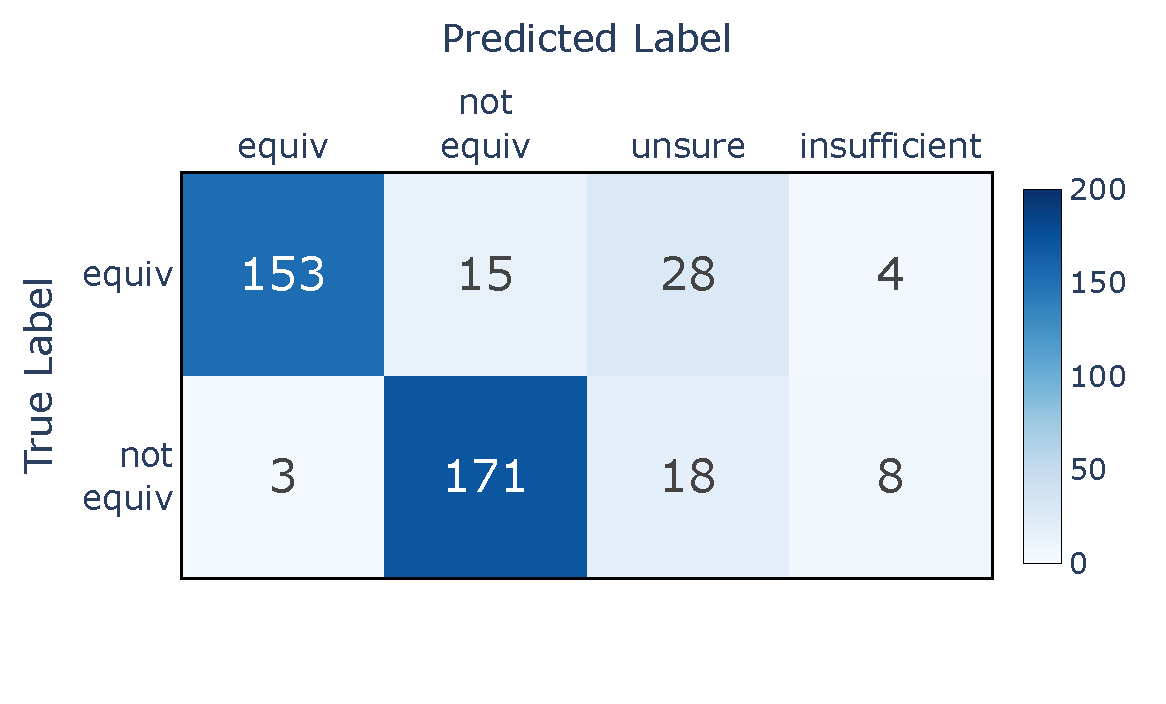
\includegraphics[scale=0.42,trim={3mm 20mm 7mm 0},clip]{LLMeval_4way_raw_text_cm.pdf}
        \caption{4-way Raw Text}
        \label{fig:sub_brt}
    \end{subfigure}
    \hfill
    \begin{subfigure}[b]{0.497\textwidth}
        \centering
        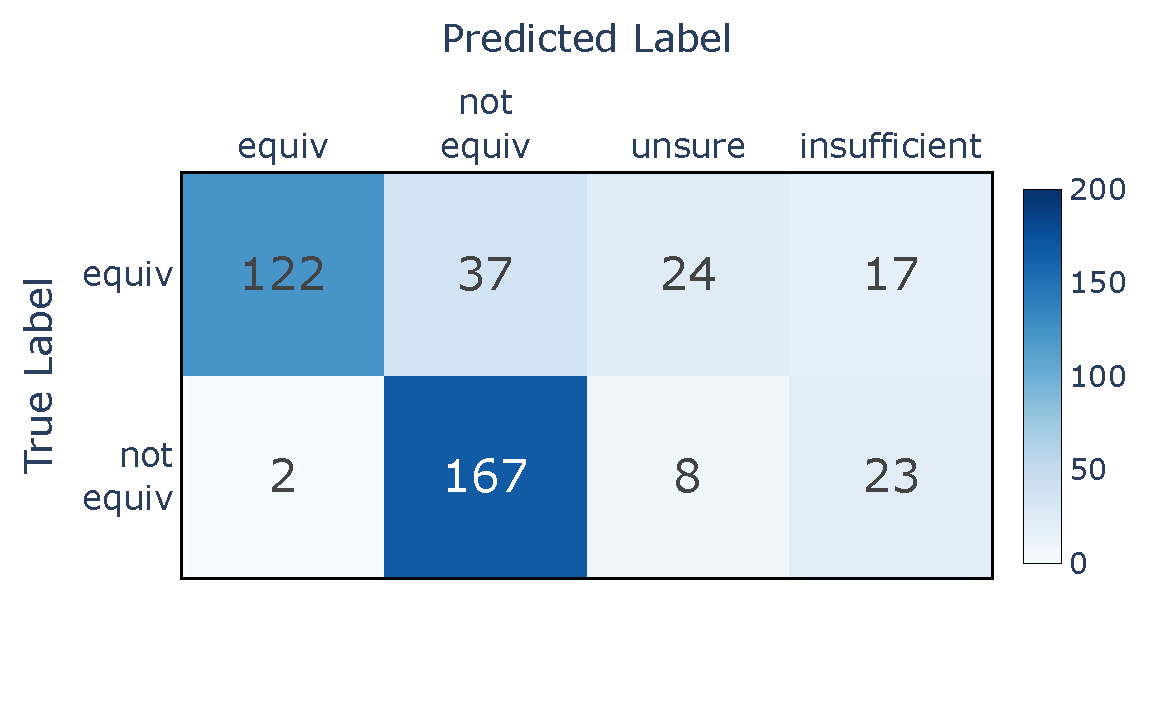
\includegraphics[scale=0.42,trim={3mm 20mm 7mm 0},clip]{LLMeval_4way_topics_cm.pdf}
        \caption{4-way Topics}
        \label{fig:sub_brt}
    \end{subfigure}
    \caption{LLM Classification Confusion Matrices}
    % {\footnotesize Clockwise from bottom left: 4-class raw text, 3-class raw text, binary raw text, binary
    %     structured topics, 3-class structured topics, and 4-class structured topics.\\\footnotemarkins: insufficient description}
    \label{fig:cm}
\end{figure}

\begin{table}[!tb]
    \captionsetup{skip=5pt}
    \centering
    \caption{Performance Summary of Direct LLM Classification}
    \label{tbl:llm_results_summary}
    \begin{tabular}{lccccc}
        \toprule
                                  & \textbf{Classification} &                   &                    &                     &                   \\
        \textbf{Input Data}       & \textbf{Task}           & \textbf{Accuracy} & \textbf{F1-Score*} & \textbf{Precision*} & \textbf{Recall*}  \\
        \midrule
        \multirow{3}{*}{Raw Text} & Binary                  & 0.9050            & 0.8973             & 0.9765              & 0.8300            \\
                                  & 3-way                   & 0.8750            & 0.8877             & 0.9818              & 0.8100            \\
                                  & 4-way                   & 0.8100            & 0.8596             & 0.9808              & 0.7650            \\
        \midrule
        \multirow{3}{*}{Topics}   & Binary                  & 0.8100            & 0.7654             & 1.0000              & 0.6200            \\
                                  & 3-way                   & 0.7775            & 0.7795             & 0.9847              & 0.6450            \\
                                  & 4-way                   & 0.7225            & 0.7531             & 0.9839              & 0.6100            \\
        \bottomrule
        \multicolumn{6}{p{0.9\textwidth}}{\scriptsize * F1-Score, Precision, and Recall are reported for the positive class (``Equivalent'').} \\
    \end{tabular}
\end{table}

\begin{table}[tb]
    \captionsetup{skip=5pt}
    \caption{Model Specifications and Performance}
    \label{tbl:cls}
    \centering
    \resizebox{\columnwidth}{!}{
        \begin{tabular}{lccccccc}
            \toprule
                                            &                      & \textbf{Context}                &                  &                   &
                                            &                      &                                                                                                                     \\
            \textbf{Model Name}             & \textbf{Parameters*} & \textbf{Length}                 & \textbf{Support} & \textbf{Accuracy} &
            \textbf{Precision}              & \textbf{Recall}      & \(\mathbf{F_1}\)\textbf{-score}                                                                                     \\
            \midrule
            Google Gemini Pro 1.0           & Unknown              & 32,768                          & 400              & \textbf{0.9050}   & 0.9765 & \textbf{0.8300} & \textbf{0.8973} \\
            Meta Llama 3.1 8B Instruct      & 8                    & 128,000                         & 208 (52\%)       & 0.6250            & 1.0000 & 0.3500          & 0.5185          \\
            Microsoft Phi 3 Medium Instruct & 14                   & 128,000                         & 400              & 0.7100            & 1.0000 & 0.4200          & 0.5915          \\
            Google Gemma 2 27b              & 27.2                 & 8,000                           & N/A              & N/A               & N/A    & N/A             & N/A             \\
            Meta Llama 3.1 70B Instruct     & 70                   & 128,000                         & 400              & 0.7350            & 1.0000 & 0.4700          & 0.6395          \\
            Qwen 2 72B Instruct             & 72.7                 & 131,072                         & 400              & 0.7650            & 1.0000 & 0.5300          & 0.6928          \\
            Anthracite Magnum v1 72B        & 72.7                 & 32,768                          & 400              & 0.8525            & 1.0000 & 0.7050          & 0.8270          \\
            CalmeRys 78B Orpo v0.1          & 78                   & 32,768                          & 400              & 0.7175            & 1.0000 & 0.4350          & 0.6063          \\
            Mixtral 8x22B Instruct v0.1     & 141                  & 65,536                          & 400              & 0.6450            & 1.0000 & 0.2900          & 0.4496          \\
            Meta Llama 3.1 405B Instruct**  & 405                  & 128,000                         & 400              & 0.7775            & 1.0000 & 0.5550          & 0.7138          \\
            \bottomrule
            \multicolumn{8}{l}{\footnotesize *in Billions}                                                                                                                               \\
            \multicolumn{8}{l}{\footnotesize **INT4 Quantized Model}
        \end{tabular}
    }
\end{table}

This initial study confirmed that while direct LLM classification can achieve high accuracy, it has fundamental limitations, including high computational cost, lack of a quantifiable similarity score, sensitivity to input quality, and an opaque, ``black box'' nature. These challenges validated the decision to pivot and motivated the development of the more robust, decoupled pipeline that is the primary focus of this thesis.

\section{Core Component Validation: The Composite Distance Vector}\label{ch:4.3}
A foundational contribution of this research is the composite distance vector, \(\Delta_c\), introduced in Section~\ref{ch:3.2.3.2}. This vector was designed to provide a richer feature set for downstream classifiers by combining granular, dimension-specific differences with a holistic, global cosine similarity metric. To validate this design, an ablation study was conducted to quantify the impact of the global cosine similarity term on classifier performance whose results are summarized in Figure~\ref{fig:ablation}. Classifiers were trained on both the complete vector (\(\Delta_c\)) and an ablated version containing only the local, element-wise differences (\(\Delta_l\)).

\begin{figure}[tb]
    \captionsetup{skip=5pt}
    \centering
    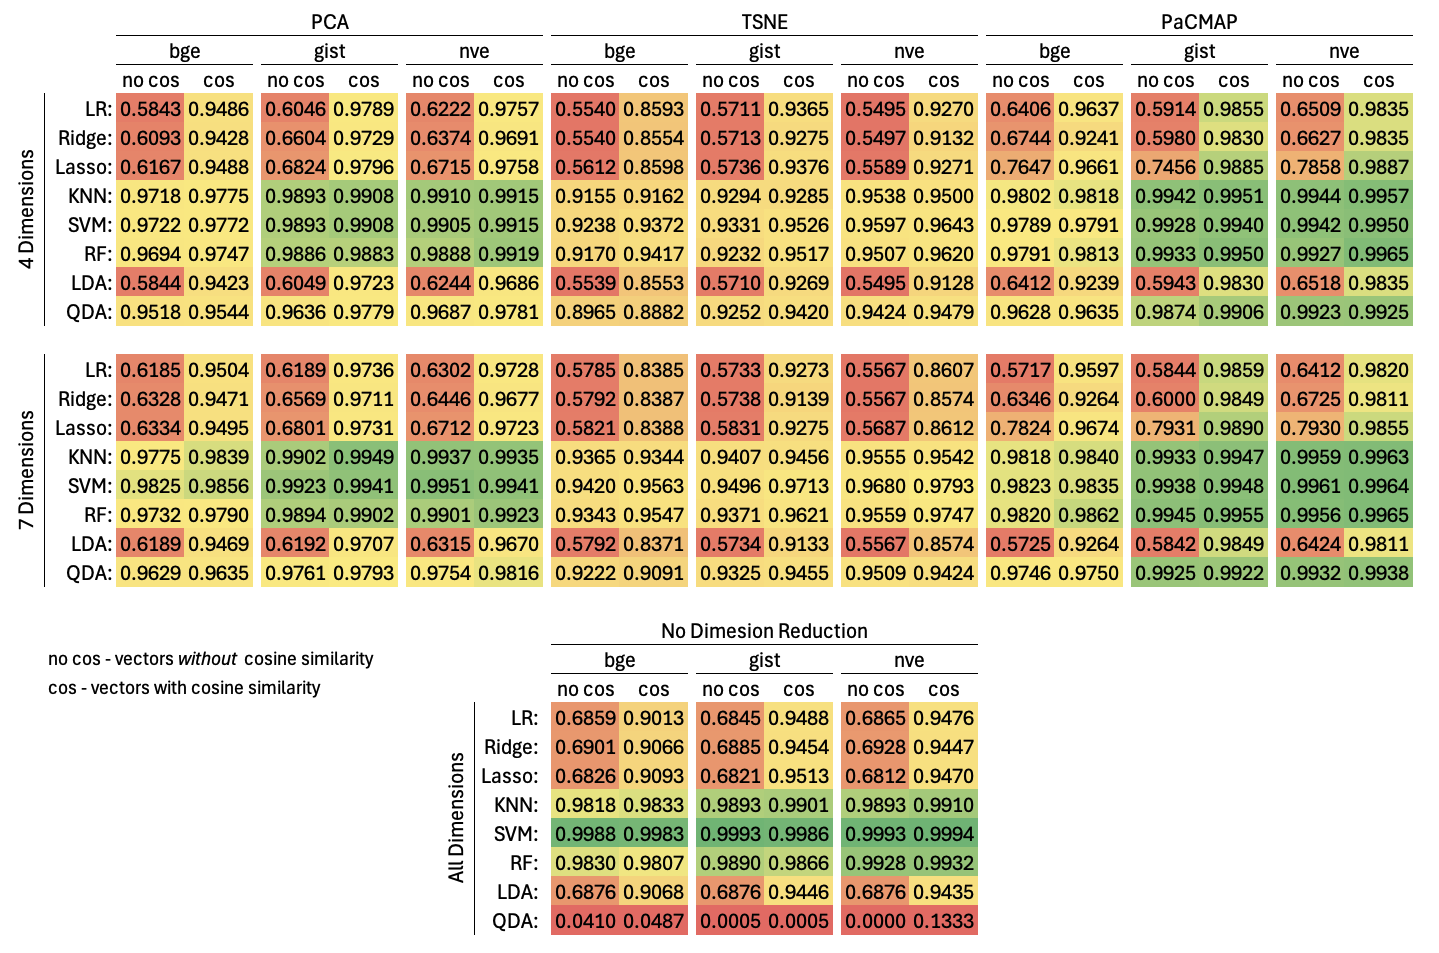
\includegraphics[width=\textwidth,trim={0 0 0 0},clip]{allcompare.png}
    \caption{A comparison of composite distance vs. elementwise-distance only.}
    \label{fig:ablation}
\end{figure}

The results revealed a stark dichotomy between the behavior of linear and non-linear models. The performance of linear models, such as Logistic Regression, showed a dramatic improvement with the inclusion of the cosine similarity term. For example, the \(F_1\)-score for Logistic Regression surged from 0.686 to 0.901 with the addition of the single global feature. This demonstrates that these simpler models, which are constrained to learning linear decision boundaries, rely on this explicit global feature and are unable to derive the relationship from the local difference vector alone. In contrast, the performance of more complex, non-linear models (e.g., KNN, SVM, and Random Forest) was not noticeably affected. Their exceptionally high performance remained stable with or without the cosine similarity term, suggesting these more powerful models are capable of inferring the global relationship directly from the high-dimensional local difference vector.

The results of this ablation study are conclusive regarding the utility of the composite distance vector, \(\Delta_c\). For linear models, its inclusion is vital, providing a substantial boost in performance. While the more powerful non-linear models did not derive a consequential benefit, their performance was not negatively impacted. Therefore, to maintain a consistent and robust feature engineering pipeline, the composite distance vector was retained as the standard feature representation for all subsequent experiments. The exploration into alternative composite vectors that could potentially yield improvements for non-linear models is an avenue for future research.

\section{Domain-Specific Adaptation: Embedding Model Fine-Tuning}\label{ch:4.4}
This section details the empirical investigation into enhancing a pre-trained embedding model by fine-tuning it on the domain-specific PPM Corpus. This process, a form of deep metric learning, aims to restructure the embedding space such that geometric distance directly corresponds to semantic similarity. Such an approach is particularly relevant for scenarios with high intra-class variance and low inter-class variance, a common characteristic of specialized domains where fine distinctions are paramount~\cite{mohan2023deepmetriclearningcomputer}.

\subsection{Fine-Tuning Experiment Summary}\label{ch:4.4.1}
To identify the optimal fine-tuning configuration, an evaluation was designed to test the impact of different loss functions and learning rate schedules on the \verb|BAAI/bge-small-en-v1.5| (BGE) base model. A matrix of twelve experimental configurations was executed, crossing the four triplet mining loss functions and three learning rate schedulers whose theoretical underpinnings were detailed in Section~\ref{ch:3.3.1.2}. The training was conducted on the POLARIS HPC cluster using a distributed data-parallel strategy. To ensure efficient and robust training, the \verb|GroupByLabelBatchSampler| was employed for effective triplet mining, and model performance was monitored at the end of each epoch using the \(F_1\)-score on a binary classification task. This was a deliberate choice to evaluate the model on its ultimate downstream application rather than the triplet loss objective itself, providing a more honest assessment of its ability to generalize.{\setlength{\emergencystretch}{5em}\par}

\subsection{Empirical Results}\label{ch:4.4.2}
The examination of the twelve fine-tuning configurations produced a rich set of performance data. Figure~\ref{fig:binaryf1} visualizes the validation \(F_1\)-score over the training process, providing a qualitative comparison of the learning dynamics for each configuration. For a more precise and formal comparison, the exact peak validation \(F_1\)-scores achieved by each configuration are summarized in Table~\ref{tab:finetune_f1_scores}.
\begin{figure}[tb]
    \captionsetup{skip=5pt}
    \centering
    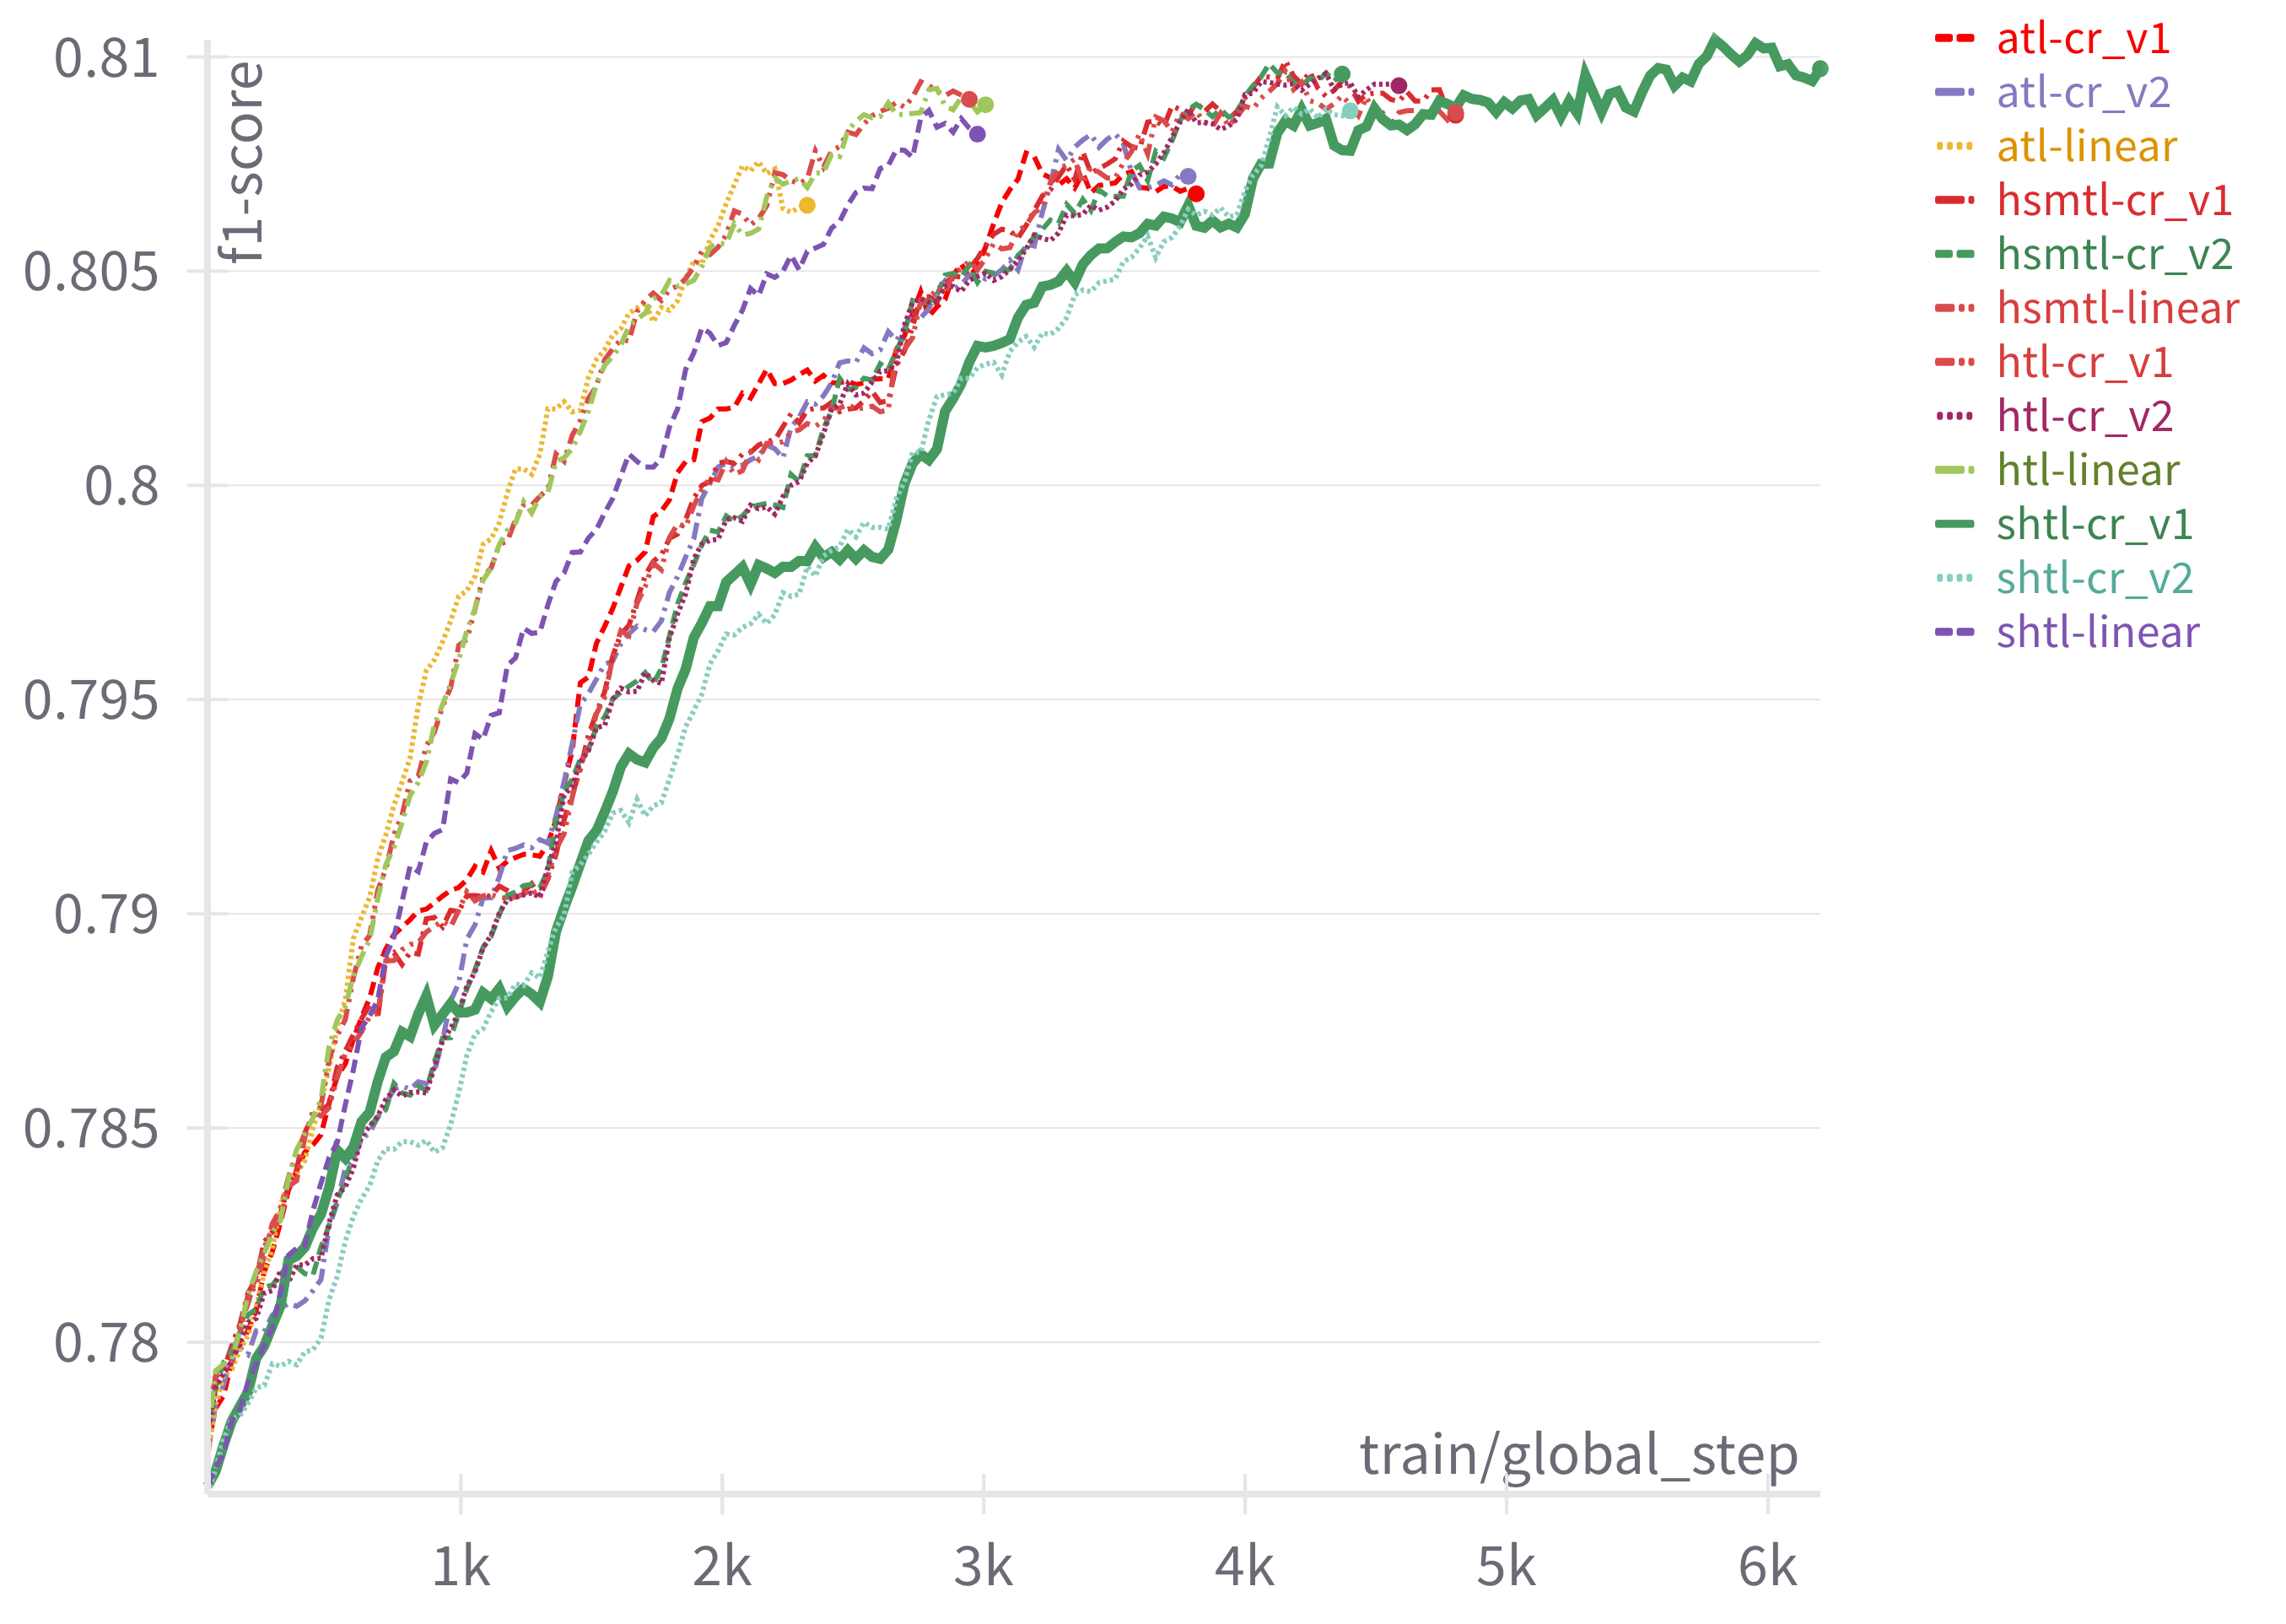
\includegraphics[scale=0.15,trim={0 0 0 0},clip]{fine-tune_validation_f1_vs_step.png}
    \caption{Validation \(F_1\)-Score}
    % {\footnotesize Clockwise from bottom left: 4-class raw text, 3-class raw text, binary raw text, binary
    %     structured topics, 3-class structured topics, and 4-class structured topics.\\\footnotemarkins: insufficient description}
    \label{fig:binaryf1}
\end{figure}
\begin{table}[tb]
    \captionsetup{skip=5pt}
    \centering
    \caption{Peak Validation F1-Score of Fine-Tuning Configurations on BGE Model}
    \label{tab:finetune_f1_scores}
    \resizebox{\columnwidth}{!}{
        \begin{tabular}{l c c c}
            \toprule
            \textbf{Loss Function}                          & \textbf{Linear Scheduler} & \textbf{Cosine Restarts v1} & \textbf{Cosine Restarts v2} \\
            \midrule
            \texttt{BatchAllTripletLoss} (atl)              & 0.8076                    & 0.8078                      & 0.8082                      \\
            \texttt{BatchHardSoftMarginTripletLoss} (hsmtl) & 0.8094                    & 0.8099                      & 0.8098                      \\
            \texttt{BatchHardTripletLoss} (htl)             & 0.8093                    & 0.8097                      & 0.8096                      \\
            \texttt{BatchSemiHardTripletLoss} (shtl)        & 0.8088                    & \textbf{0.8104}             & 0.8088                      \\
            \bottomrule
        \end{tabular}
    }
\end{table}

The quantitative data reveals a nuanced outcome. While aggressive hard-negative mining strategies such as \verb|BatchHardTripletLoss| and \verb|BatchHardSoftMarginTripletLoss| consistently provided a high performance floor, the single best-performing configuration was the combination of \verb|BatchSemiHardTripletLoss| with the \verb|cr_v1| cosine annealing schedule, which achieved the highest peak validation \(F_1\)-score of 0.8104. This result suggests that a more moderate mining strategy, when paired with a patient and robust optimization schedule, can find a slightly better optimum for this specific task.

\subsection{Validation and Selection of the Optimal Embedding Model}\label{ch:4.4.3}
The superior performance of the winning configuration arises from a synergistic framework: a stable learning objective from semi-hard mining, a robust exploration strategy from the \verb|CosineAnnealingWarmRestarts| scheduler that allows the optimizer to escape local minima, and effective regularization from the AdamW optimizer~\cite{loshchilov2019decoupledweightdecayregularization, hermans2017defensetripletlossperson, Schroff_2015, loshchilovhutter}. To definitively validate the benefit of this fine-tuning process, the performance of the resulting model (BGE-ft) was compared against the suite of off-the-shelf models using the held-out test portion of the PPM Corpus. The descriptive statistics in Table~\ref{tbl:desc_stats_embedding_model} show that the fine-tuned BGE-ft model not only achieved the highest mean \(F_1\) test score (\(\mu = 0.9787\)) but also exhibited the lowest standard deviation (\(\sigma = 0.0043\)), indicating it is both more accurate and more consistent on unseen data.

\begin{table}[!ht]
    \captionsetup{skip=5pt}
\centering
\caption{Descriptive Statistics for F1-Scores by Embedding Model (Test Data)}
\label{tbl:desc_stats_embedding_model}
\resizebox{\columnwidth}{!} & \textbf{50\%} & \textbf{75\%} & \textbf{max} \\
\midrule
BGE & 64.0 & 0.967681 & 0.015185 & 0.900304 & 0.957357 & 0.973832 & 0.978318 & 0.984612 \\
BGE-ft & 63.0 & 0.978746 & 0.004320 & 0.968707 & 0.976240 & 0.979922 & 0.981683 & 0.987702 \\
GIST & 63.0 & 0.971851 & 0.012516 & 0.913939 & 0.965367 & 0.977210 & 0.981077 & 0.984083 \\
NVE & 64.0 & 0.970530 & 0.013705 & 0.937957 & 0.960745 & 0.975147 & 0.982084 & 0.985258 \\
NVE & 64.0 & 0.972254 & 0.014617 & 0.922104 & 0.963553 & 0.978764 & 0.982926 & 0.986549 \\
\bottomrule
\end{tabular}%
}
\end{table}

To determine if these observed performance differences were statistically significant, a formal hypothesis testing procedure was conducted. First, Levene's test was performed to check the assumption of homogeneity of variances across the embedding model groups. As shown in Table~\ref{tbl:levene_embedding_model}, the result was statistically significant (\(p < 0.001\)), indicating that the variances were unequal and justifying the use of a Welch's ANOVA and the more robust Games-Howell post-hoc test. A one-way Welch's ANOVA subsequently confirmed that a statistically significant difference exists between the model groups (\(F(4, 141.9) = 15.9881, p < 0.001\)), as detailed in Table~\ref{tbl:anova_embedding_model}.

\begin{table}[tb]
    \captionsetup{skip=5pt}
\centering
\caption{Statistical Tests for F1-Scores by Embedding Model (Test Data)}
\label{tbl:stats_embedding_model}
\begin{subtable}{\linewidth}
\centering
\caption{Levene's Test for Homogeneity of Variances}
\label{tbl:levene_embedding_model}
\begin{tabular}{ccc}
\toprule
\textbf{Statistic (W)} & \textbf{df} & \textbf{p-value} \\
\midrule
7.0286 & (4, 313) & <0.001 \\
\bottomrule
\end{tabular}
\end{subtable}%
\vspace{1em}
\begin{subtable}{\linewidth}
\centering
\caption{Welch's ANOVA}
\label{tbl:anova_embedding_model}
\begin{tabular}{cccc}
\toprule
\textbf{F-statistic} & \textbf{df1} & \textbf{df2} & \textbf{p-value} \\
\midrule
15.9881 & 4 & 141.90 & <0.001 \\
\bottomrule
\end{tabular}
\end{subtable}
\end{table}

The Games-Howell post-hoc test (Table~\ref{tbl:games_howell_embedding_model}) provided detailed pairwise comparisons, revealing that the BGE-ft model demonstrated a statistically significant improvement over its base model, BGE, with a mean \(F_1\)-score increase of 0.0111 (\(p<0.001\)). Notably, BGE-ft outperformed all other evaluated models by a considerable amount, including those that were orders of magnitude larger, such as NVE and NVE. This rigorous evaluation leads to a clear and unambiguous conclusion. The single best model for this task is the \verb|BAAI/bge-small-en-v1.5| model fine-tuned using \verb|BatchSemiHardTripletLoss| and a \verb|CosineAnnealingWarmRestarts| learning rate schedule. This model, was proven to be statistically superior to all off-the-shelf models evaluated in this study and is carried forward as the primary fine-tuned embedding model for the comprehensive classifier evaluation detailed in the next section.{\setlength{\emergencystretch}{5em}\par}

\begin{table}[tb]
    \captionsetup{skip=5pt}
\centering
\caption{Games-Howell Post-Hoc Test for Embedding Models (Test Data)}
\label{tbl:games_howell_embedding_model}
        \begin{tabular}{llrrrrr}
            \toprule
             &  & \textbf{Mean} &  & \textbf{95\% CI} & \textbf{95\% CI} & \\
            \textbf{Group 1} & \textbf{Group 2} & \textbf{Diff.} & \textbf{p-adj} & \textbf{Lower} & \textbf{Upper} & \textbf{Reject}\\
\midrule
KNN & RF & -0.0007 & 0.9923 & -0.0068 & 0.0054 & False \\
KNN & SVM & 0.0051 & 0.0577 & -0.0001 & 0.0102 & False \\
KNN & XGB & -0.0001 & 0.9999 & -0.0058 & 0.0056 & False \\
RF & SVM & 0.0057 & 0.0178 & 0.0007 & 0.0107 & True \\
RF & XGB & 0.0005 & 0.9944 & -0.0050 & 0.0061 & False \\
SVM & XGB & -0.0052 & 0.0160 & -0.0097 & -0.0007 & True \\
\bottomrule
\end{tabular}
\end{table}

\section{Downstream Classifier Performance}\label{ch:4.5}
This section presents the definitive evaluation of the downstream classifiers, representing the final component of the proposed framework. The objective is to identify the optimal classification model by balancing predictive accuracy against computational efficiency. The evaluation proceeds from a broad preliminary review to a focused analysis of four finalist classifiers on the PPM Corpus, culminating in a statistical comparison on held-out test data.

\subsection{The Impact of Dimensionality Reduction}\label{ch:4.5.1}
Before evaluating the final classifiers, it is crucial to analyze the impact of the dimensionality reduction techniques detailed in Section~\ref{ch:3.2.3.1}. The high-dimensional vectors produced by embedding models can pose challenges for some classifiers, and reducing dimensionality can potentially improve performance and efficiency. A comprehensive statistical analysis was performed on the test data to compare the efficacy of using the original embeddings versus those transformed by PCA, UMAP, and PaCMAP, as well as to compare different target dimensionalities.

The results, summarized in Tables~\ref{tbl:desc_stats_dim_reducer} through~\ref{tbl:games_howell_num_dim}, reveal a clear and pronounced finding: dimensionality reduction is not just a computational optimization but a key step for improving classification accuracy. The PaCMAP reducer, in particular, stands out, achieving a statistically significant improvement over all other methods, including using no reduction at all (\(p<0.05\) for all comparisons).Nevetheless, a particular item of note is that BGE-ft performed the best while using PCA.  Similarly, when analyzing the target number of dimensions, reducing the feature space to a size that explains 70\% or 80\% of the original variance yields a statistically significant performance boost over using the original embeddings or reducing to a very small, fixed number of dimensions like 5. These results strongly suggest that dimensionality reduction techniques, particularly PaCMAP and PCA, effectively filter noise and distill the most discriminative signals from the high-dimensional embeddings, leading to a more robust feature set for the downstream classifiers. All subsequent classifier evaluations, therefore, incorporate these optimized, dimensionally-reduced feature vectors.

\begin{table}[!ht]
    \captionsetup{skip=5pt}
\centering
\caption{Descriptive Statistics for F1-Scores by Dimensionality Reducer (Test Data)}
\label{tbl:desc_stats_dim_reducer}
\resizebox{\columnwidth}{!} & \textbf{50\%} & \textbf{75\%} & \textbf{max} \\
\midrule
None & 20.0 & 0.962981 & 0.024292 & 0.900304 & 0.961691 & 0.972235 & 0.976458 & 0.983663 \\
pacmap & 98.0 & 0.981104 & 0.001835 & 0.977172 & 0.979452 & 0.981442 & 0.982431 & 0.984393 \\
pca & 100.0 & 0.971991 & 0.012743 & 0.937957 & 0.962466 & 0.977626 & 0.982058 & 0.987702 \\
umap & 100.0 & 0.965505 & 0.011596 & 0.938061 & 0.956572 & 0.968961 & 0.974924 & 0.982183 \\
\bottomrule
\end{tabular}%
}
\end{table}

\begin{table}[!ht]
    \captionsetup{skip=5pt}
\centering
\caption{Games-Howell Post-Hoc Test for Dimensionality Reducers (Test Data)}
\label{tbl:games_howell_dim_reducer_full}
        \begin{tabular}{llrrrrr}
            \toprule
             &  & \textbf{Mean} &  & \textbf{95\% CI} & \textbf{95\% CI} & \\
            \textbf{Group 1} & \textbf{Group 2} & \textbf{Diff.} & \textbf{p-adj} & \textbf{Lower} & \textbf{Upper} & \textbf{Reject}\\
\midrule
None & PaCMAP & 0.0181 & 0.0167 & 0.0028 & 0.0334 & True \\
None & PCA & 0.0090 & 0.3920 & -0.0065 & 0.0246 & False \\
None & UMAP & 0.0025 & 0.9680 & -0.0130 & 0.0180 & False \\
PaCMAP & PCA & -0.0091 & <0.001 & -0.0125 & -0.0058 & True \\
PaCMAP & UMAP & -0.0156 & <0.001 & -0.0187 & -0.0125 & True \\
PCA & UMAP & -0.0065 & 0.0013 & -0.0110 & -0.0020 & True \\
\bottomrule
\end{tabular}
\end{table}

\begin{table}[!ht]
    \captionsetup{skip=5pt}
\centering
\caption{Descriptive Statistics for F1-Scores by Number of Dimensions (Test Data)}
\label{tbl:desc_stats_num_dim}
\resizebox{\columnwidth}{!} & \textbf{50\%} & \textbf{75\%} & \textbf{max} \\
\midrule
5 & 60.0 & 0.966575 & 0.014254 & 0.937957 & 0.955814 & 0.969970 & 0.980417 & 0.983850 \\
7 & 59.0 & 0.970692 & 0.009840 & 0.950073 & 0.962735 & 0.972467 & 0.980017 & 0.983124 \\
70\% & 60.0 & 0.975803 & 0.009528 & 0.944029 & 0.973550 & 0.979290 & 0.982021 & 0.985604 \\
80\% & 60.0 & 0.976336 & 0.009952 & 0.938061 & 0.975156 & 0.979441 & 0.982494 & 0.986549 \\
90\% & 59.0 & 0.974646 & 0.012442 & 0.939868 & 0.974690 & 0.979041 & 0.982269 & 0.987702 \\
Original & 20.0 & 0.962981 & 0.024292 & 0.900304 & 0.961691 & 0.972235 & 0.976458 & 0.983663 \\
\bottomrule
\end{tabular}%
}
\end{table}

\begin{table}[!ht]
    \captionsetup{skip=5pt}
\centering
\caption{Games-Howell Post-Hoc Test for Number of Dimensions (Test Data)}
\label{tbl:games_howell_num_dim}
        \begin{tabular}{llrrrrr}
            \toprule
             &  & \textbf{Mean} &  & \textbf{95\% CI} & \textbf{95\% CI} & \\
            \textbf{Group 1} & \textbf{Group 2} & \textbf{Diff.} & \textbf{p-adj} & \textbf{Lower} & \textbf{Upper} & \textbf{Reject}\\
\midrule
5 & 7 & 0.0041 & 0.4473 & -0.0024 & 0.0106 & False \\
5 & 70\% & 0.0092 & 0.0009 & 0.0028 & 0.0157 & True \\
5 & 80\% & 0.0098 & 0.0004 & 0.0032 & 0.0163 & True \\
5 & 90\% & 0.0081 & 0.0162 & 0.0010 & 0.0152 & True \\
5 & Original & -0.0036 & 0.9878 & -0.0214 & 0.0142 & False \\
7 & 70\% & 0.0051 & 0.0527 & -0.0000 & 0.0103 & False \\
7 & 80\% & 0.0056 & 0.0277 & 0.0004 & 0.0109 & True \\
7 & 90\% & 0.0040 & 0.3988 & -0.0020 & 0.0099 & False \\
7 & Original & -0.0077 & 0.7370 & -0.0252 & 0.0097 & False \\
70\% & 80\% & 0.0005 & 0.9997 & -0.0046 & 0.0057 & False \\
70\% & 90\% & -0.0012 & 0.9928 & -0.0071 & 0.0047 & False \\
70\% & Original & -0.0128 & 0.2368 & -0.0302 & 0.0046 & False \\
80\% & 90\% & -0.0017 & 0.9638 & -0.0077 & 0.0043 & False \\
80\% & Original & -0.0134 & 0.2033 & -0.0308 & 0.0041 & False \\
90\% & Original & -0.0117 & 0.3432 & -0.0293 & 0.0060 & False \\
\bottomrule
\end{tabular}
\end{table}

\subsection{Efficacy vs. Efficiency Analysis}\label{ch:4.5.2}
With the feature set optimized, the analysis next investigated the trade-off between model efficacy and computational efficiency for the four finalist classifiers: K-Nearest Neighbors (KNN), Support Vector Machine (SVM), Random Forest (RF), and XGBoost. Figure~\ref{fig:f1time} visualizes the median \(F_1\)-scores from the cross-validation grid search against both training and inference times.  While all four models demonstrate the ability to achieve high accuracy, Random Forest and XGBoost emerge as the clear winners with respect to inference time.  Their inference times are tightly clustered under 0.1 seconds---an order of magnitude faster and more predictable than the wider, more variable times of KNN and SVM.  This reliability makes RF and XGBoost inherently more robust choices for a scalable, low-latency production system.
\begin{figure}[tb]
    \captionsetup{skip=5pt}
    \centering
    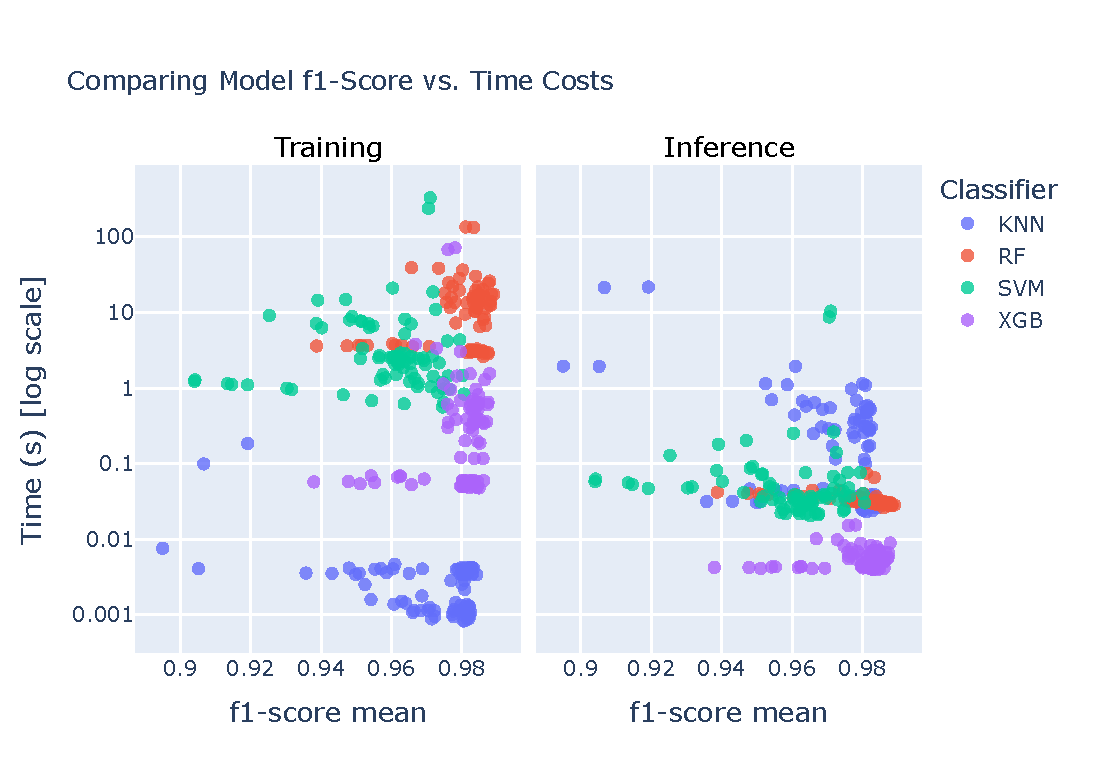
\includegraphics[scale=0.85,trim={0 5mm 0 18mm},clip]{cv_f1 vs time.pdf}
    \caption{Classifier \(F_1\)-Score vs. Training and Inference Time}
    \label{fig:f1time}
\end{figure}

\subsection{Statistical Analysis of Classifier Performance on Test Data}\label{ch:4.5.3}
The definitive comparison was conducted on the held-out test data from the PPM Corpus. As shown in the score distributions (Figure~\ref{fig:clscoredist}) and descriptive statistics (Table~\ref{tbl:desc_stats_classifier}), all four classifiers demonstrate exceptionally high and stable performance. To provide a more comprehensive view of classifier performance beyond the \(F_1\)-score, Receiver Operating Characteristic (ROC) curves were generated, as shown in Figure~\ref{fig:roc_unzoomed}. The Area Under the Curve (AUC) scores for all models are exceptionally high (all \(>0.98\)), indicating excellent discrimination capability across all classification thresholds. The zoomed-in Figure~\ref{fig:roc_zoomed} highlights the subtle but consistent superiority of the SVM model. Further visualization through confusion matrices (Figure~\ref{fig:classifier_cms}) for the best-performing hyperparameter configuration of each classifier paired with BGE-ft confirms their strong performance, with very few misclassifications overall. For more detailed ROC curves and confusion matrices for every embedding model, see Appendix~\ref{app:roc_cm}.

\begin{figure}[tb]
    \captionsetup{skip=5pt}
    \centering
    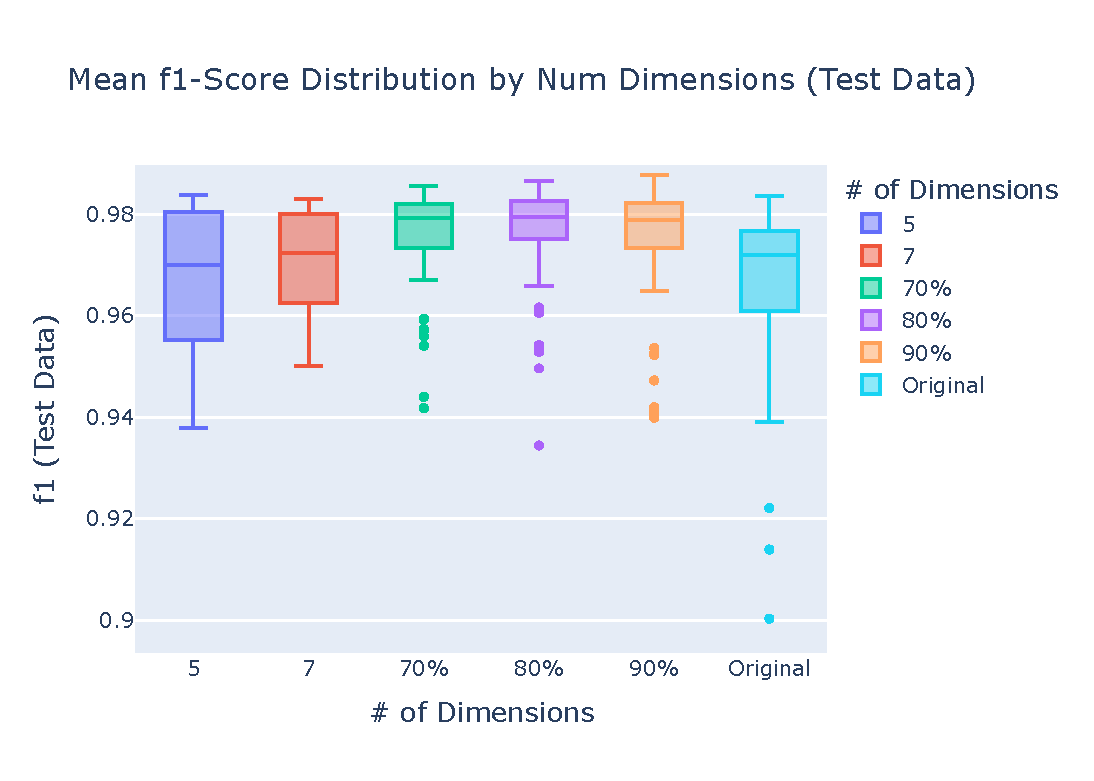
\includegraphics[scale=0.75,trim={0 5mm 0 18mm},clip]{classifier_f1score_boxplot_test.pdf}
    \caption{\(F_1\)-Score Distribution of Finalist Classifiers}
    \label{fig:clscoredist}
\end{figure}

\begin{table}[tb]
    \captionsetup{skip=5pt}
    \caption{Classifier Descriptive Statistics on Test Data F1-Scores}
    \label{tbl:desc_stats_classifier}
    \centering
    \resizebox{\columnwidth}{!}{
        \begin{tabular}{lcccccccc}
            \toprule                                                          
            \textbf{Classifier} & \textbf{Count} & \textbf{Mean} & \textbf{Std} & \textbf{Min} & \textbf{25\%} & \textbf{50\%} & \textbf{75\%} & \textbf{Max} \\
            \midrule
            KNN & 80.0 & 0.971147 & 0.015208 & 0.900304 & 0.971809 & 0.977110 & 0.979110 & 0.982437 \\
            RF & 80.0 & 0.970490 & 0.014473 & 0.938061 & 0.957396 & 0.978490 & 0.982073 & 0.984572 \\
            SVM & 78.0 & 0.976210 & 0.009112 & 0.939885 & 0.970793 & 0.979567 & 0.982795 & 0.987702 \\
            XGB & 80.0 & 0.971026 & 0.012316 & 0.942860 & 0.959382 & 0.977547 & 0.981376 & 0.984898 \\
            \bottomrule
        \end{tabular}
    }
\end{table}

\begin{figure}[tb]
    \captionsetup{skip=5pt}
    \centering
    \captionsetup[subfigure]{oneside,margin={1cm,0cm}}
    \subfloat[Zoomed]{
        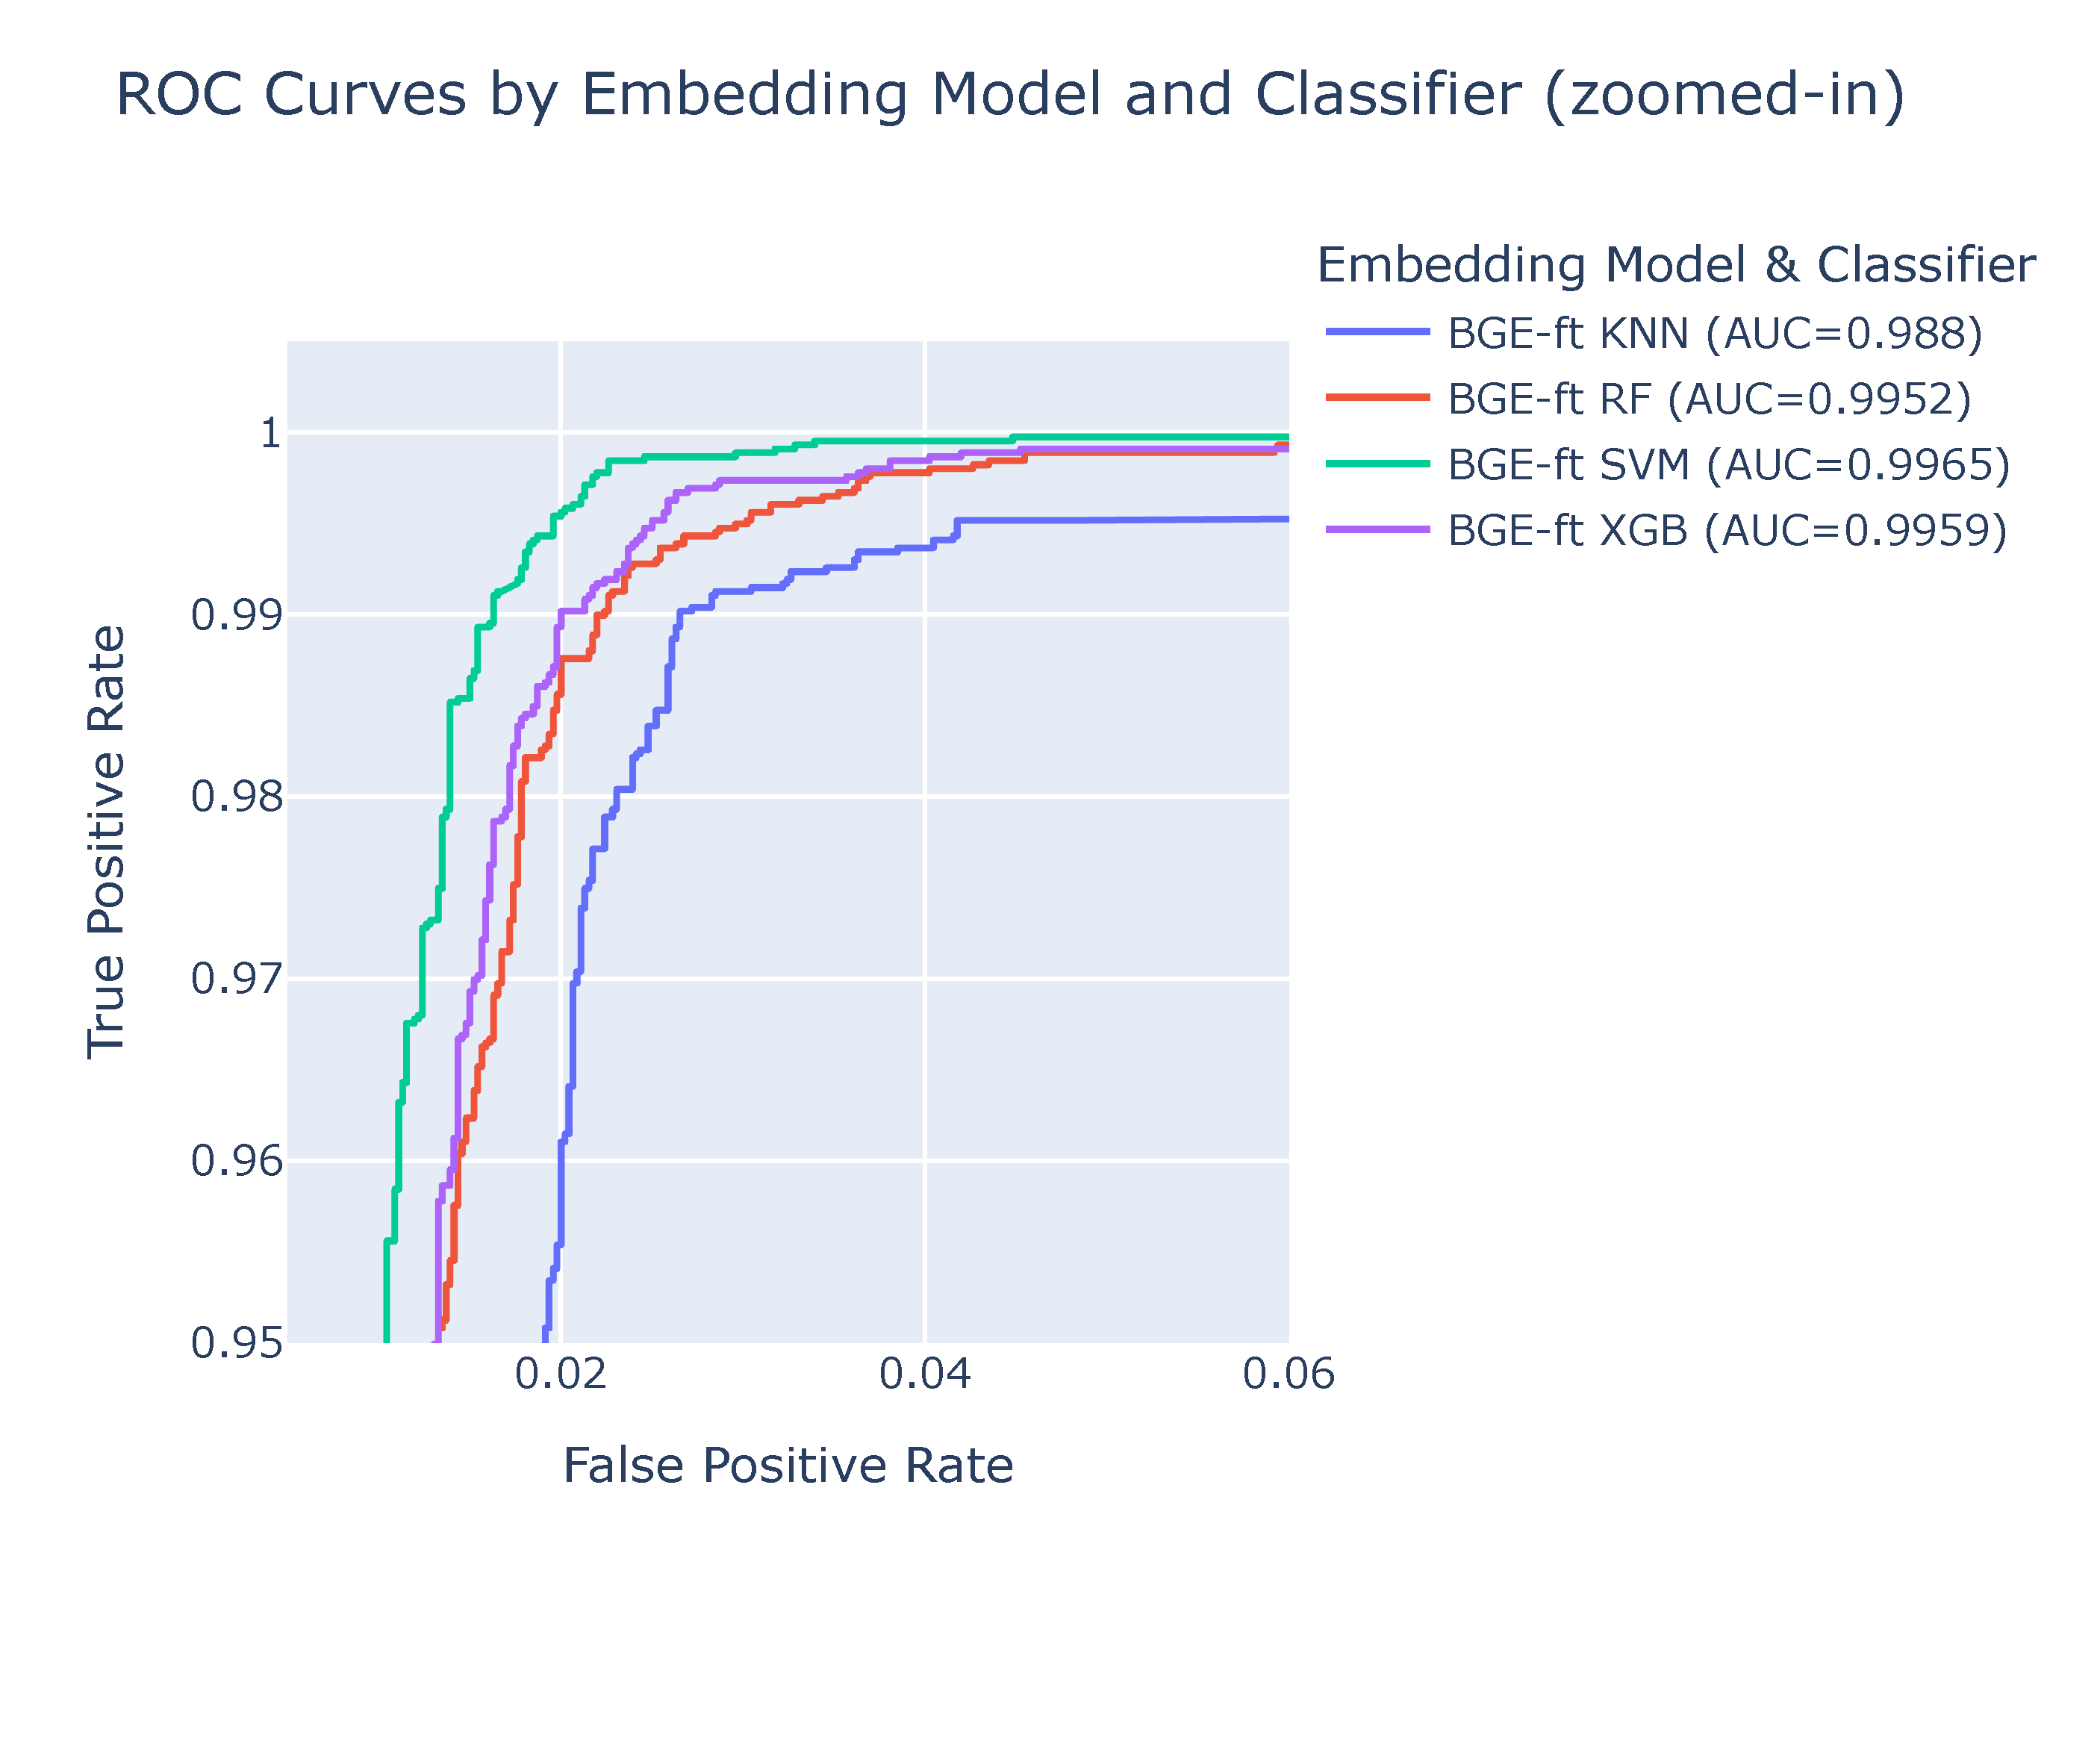
\includegraphics[width=0.37\textwidth,trim={18mm 50mm 180mm 50mm},clip]{roc_curves_bgeft_zoomed.pdf}\label{fig:roc_zoomed}
    }
    \captionsetup[subfigure]{oneside,margin={-2.5cm,0cm}}
    \subfloat[Full Size]{
        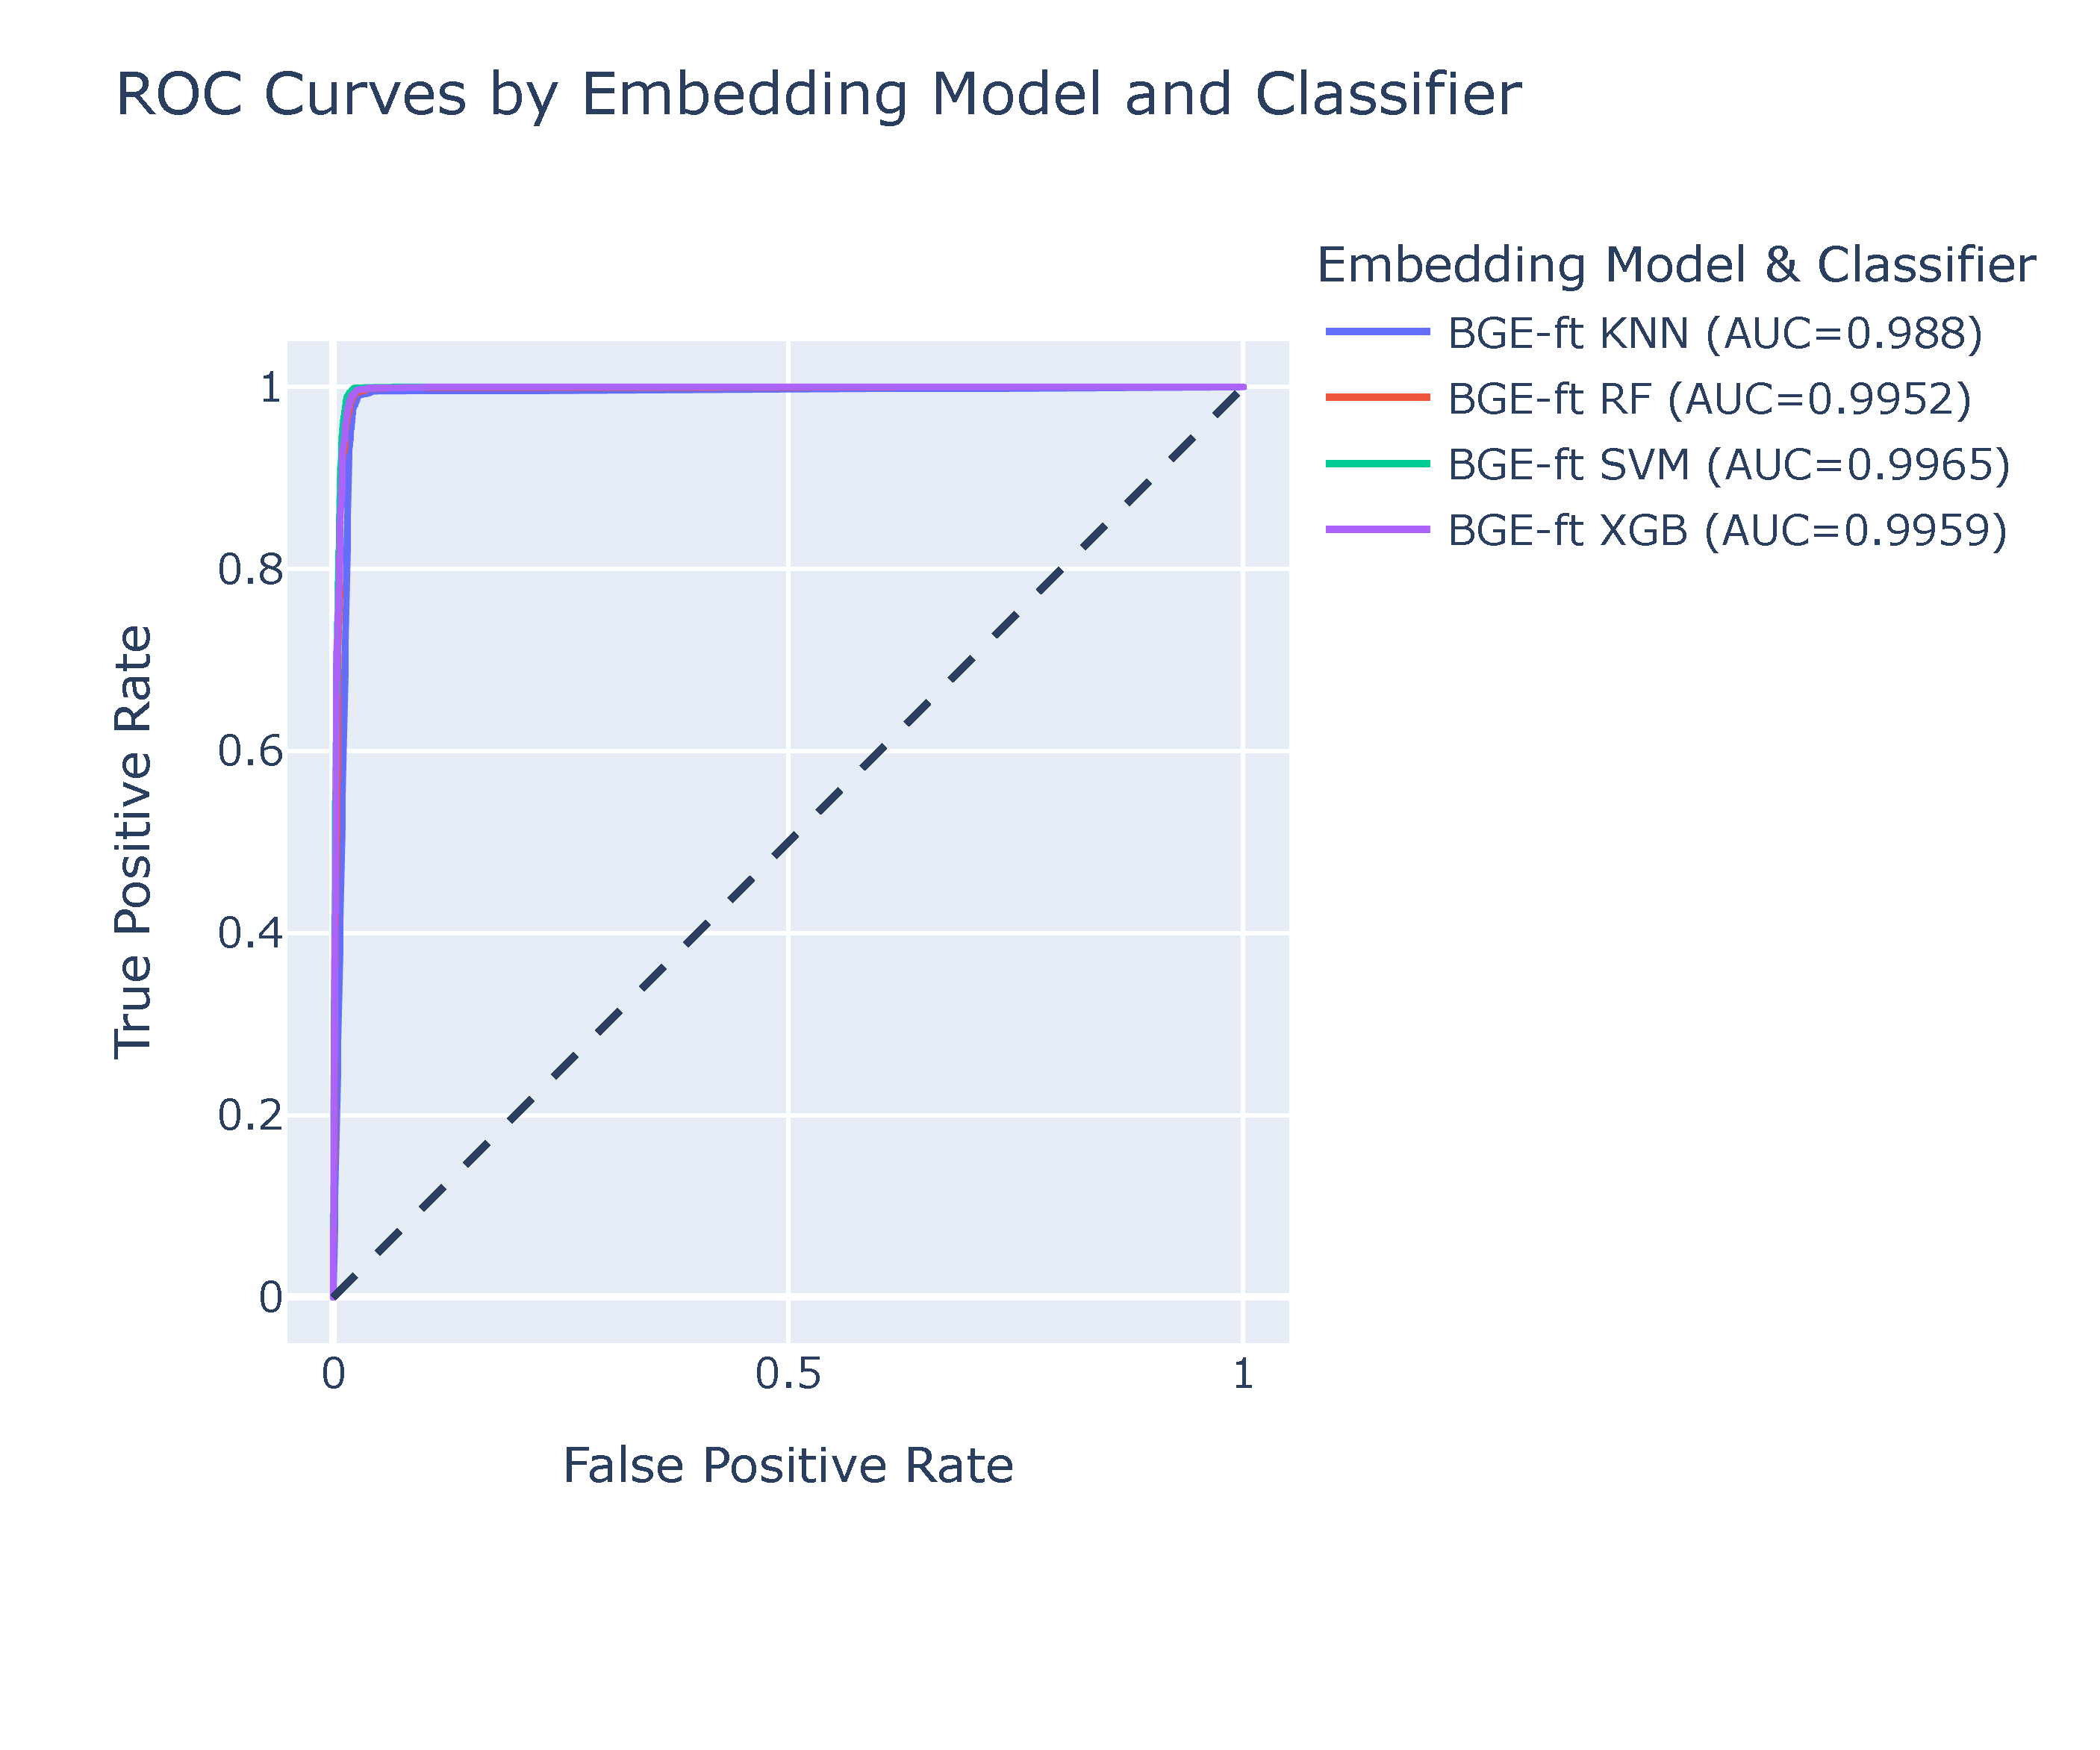
\includegraphics[width=0.58\textwidth,trim={25mm 50mm 12mm 50mm},clip]{roc_curves_bgeft.pdf}\label{fig:roc_unzoomed}
    }
    \caption{BGE-ft ROC Curves for Finalist Classifiers with Test Data}
\end{figure}

\begin{figure}[tb]
    \captionsetup{skip=5pt}
    \centering
    \captionsetup[subfigure]{oneside,margin={1.3cm,0cm}}
    \subfloat[KNN]{
        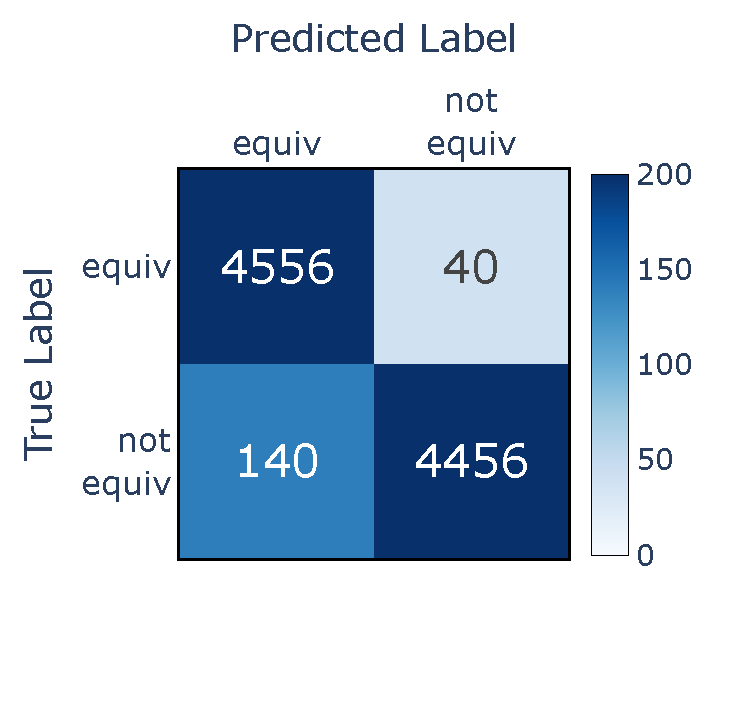
\includegraphics[width=0.277\textwidth,trim={0 23mm 26mm 0},clip]{cm_BGE-ft_pacmap_knn.pdf}\label{fig:cm_knn}
    }
    \captionsetup[subfigure]{oneside,margin={0cm,0cm}}
    \subfloat[Random Forest]{
        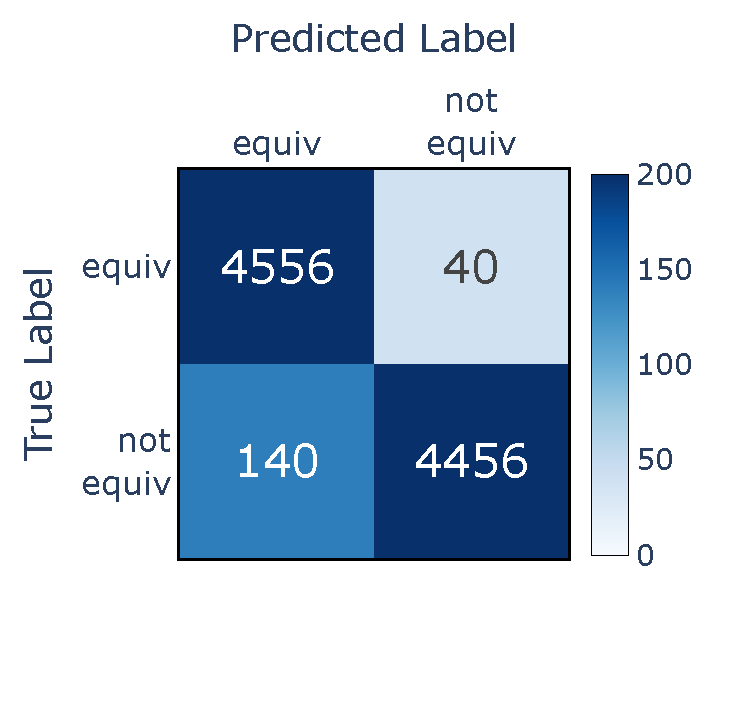
\includegraphics[width=0.194\textwidth,trim={29mm 23mm 26mm 0},clip]{cm_BGE-ft_pca_rf.pdf}\label{fig:cm_rf}
    }
    \captionsetup[subfigure]{oneside,margin={0cm,0cm}}
    \subfloat[SVM]{
        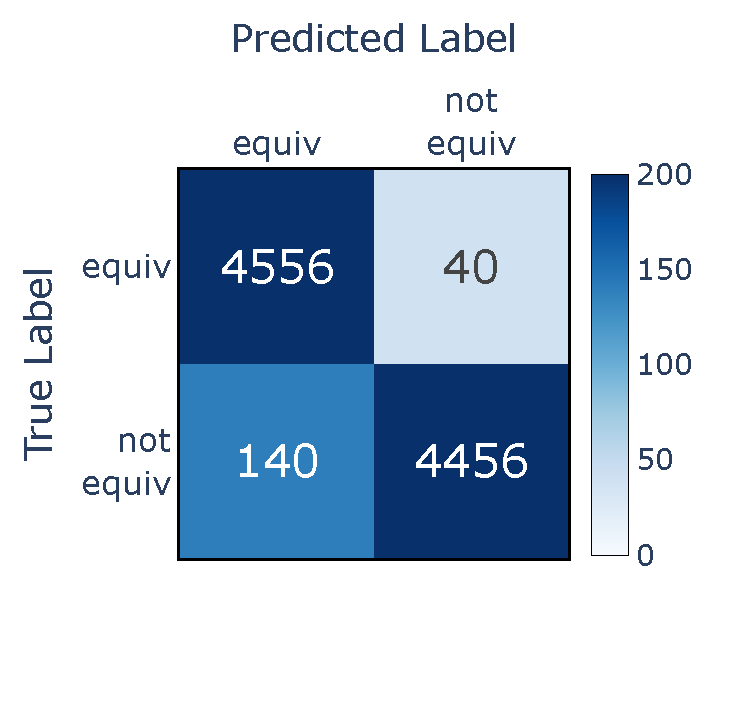
\includegraphics[width=0.194\textwidth,trim={29mm 23mm 26mm 0},clip]{cm_BGE-ft_pca_svm.pdf}\label{fig:cm_svm}
    }
    \captionsetup[subfigure]{oneside,margin={-1.25cm,0cm}}
    \subfloat[XGBoost]{
        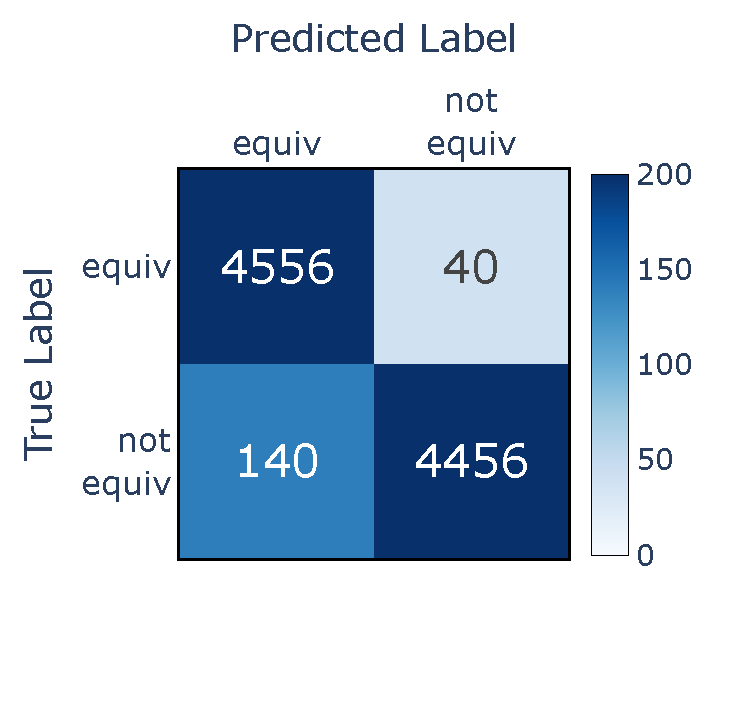
\includegraphics[width=0.246\textwidth,trim={29mm 23mm 7mm 0},clip]{cm_BGE-ft_pca_xgb.pdf}\label{fig:cm_xgb}
    }
    \caption{BGE-ft Confusion Matrices for Finalist Classifiers with Test Data}
    \label{fig:classifier_cms}
\end{figure}

Notably, the Support Vector Machine (SVM) model achieved both the highest mean \(F_1\)-score (\(\mu = 0.9762\)) and the lowest standard deviation (\(\sigma = 0.0091\)), indicating it is the most accurate and consistent performer. To determine if these observed differences were statistically significant, a one-way Welch's ANOVA was performed, which confirmed a significant difference among the classifiers (\(F(3, 171.4) = 5.0484, p = 0.0022\)). A subsequent Games-Howell post-hoc test, justified due to unequal variances confirmed by Levene's Test (\(p=0.0387\)), revealed that the SVM classifier performed statistically significantly better than both Random Forest (mean difference \(= 0.0057, p=0.0178\)) and XGBoost (mean difference \(= 0.0052, p=0.016\)). While all four are top-tier performers, the formal statistical analysis identifies SVM as the definitive winner in terms of raw accuracy. The full statistical results are presented in Tables~\ref{tbl:desc_stats_classifier} and~\ref{tbl:games_howell_classifier_full}.

\begin{table}[tb]
    \captionsetup{skip=5pt}
    \caption{Classifier Descriptive Statistics on Test Data F1-Scores}
    \label{tbl:desc_stats_classifier}
    \centering
    \resizebox{\columnwidth}{!}{
        \begin{tabular}{lcccccccc}
            \toprule                                                          
            \textbf{Classifier} & \textbf{Count} & \textbf{Mean} & \textbf{Std} & \textbf{Min} & \textbf{25\%} & \textbf{50\%} & \textbf{75\%} & \textbf{Max} \\
            \midrule
            KNN & 80.0 & 0.971147 & 0.015208 & 0.900304 & 0.971809 & 0.977110 & 0.979110 & 0.982437 \\
            RF & 80.0 & 0.970490 & 0.014473 & 0.938061 & 0.957396 & 0.978490 & 0.982073 & 0.984572 \\
            SVM & 78.0 & 0.976210 & 0.009112 & 0.939885 & 0.970793 & 0.979567 & 0.982795 & 0.987702 \\
            XGB & 80.0 & 0.971026 & 0.012316 & 0.942860 & 0.959382 & 0.977547 & 0.981376 & 0.984898 \\
            \bottomrule
        \end{tabular}
    }
\end{table}

\begin{table}[tb]
    \captionsetup{skip=5pt}
\centering
\caption{Games-Howell Post-Hoc Test for Classifiers (Test Data)}
\label{tbl:games_howell_classifier_full}
        \begin{tabular}{llrrrrr}
            \toprule
             &  & \textbf{Mean} &  & \textbf{95\% CI} & \textbf{95\% CI} & \\
            \textbf{Group 1} & \textbf{Group 2} & \textbf{Diff.} & \textbf{p-adj} & \textbf{Lower} & \textbf{Upper} & \textbf{Reject}\\
\midrule
KNN & RF & -0.0007 & 0.9923 & -0.0068 & 0.0054 & False \\
KNN & SVM & 0.0051 & 0.0577 & -0.0001 & 0.0102 & False \\
KNN & XGB & -0.0001 & 0.9999 & -0.0058 & 0.0056 & False \\
RF & SVM & 0.0057 & 0.0178 & 0.0007 & 0.0107 & True \\
RF & XGB & 0.0005 & 0.9944 & -0.0050 & 0.0061 & False \\
SVM & XGB & -0.0052 & 0.0160 & -0.0097 & -0.0007 & True \\
\bottomrule
\end{tabular}
\end{table}

\subsection{Final Classifier Selection}\label{ch:4.5.4}
This multi-stage evaluation reveals a classic trade-off between peak performance and operational efficiency. The statistical superiority of SVM is clear; however, it corresponds to a mean \(F_1\)-score improvement of only about 0.5\% over the far more efficient tree-based models. The final choice is therefore context-dependent. Based on the comprehensive evidence, the following recommendations are made:
\begin{itemize}
    \item \textbf{For Maximum Accuracy}: The Support Vector Machine (SVM) is the recommended classifier for any scenario where achieving the absolute highest accuracy and consistency is the paramount objective.
    \item \textbf{For Optimal Efficiency}: Random Forest and XGBoost are compelling and practical alternatives for applications where inference speed, low latency, and predictable performance are essential for scalability. They provide nearly equivalent accuracy with demonstrably superior and more reliable computational efficiency.
\end{itemize}

\section{Qualitative Diagnosis: Misclassification Analysis}\label{ch:4.6}
While quantitative metrics are essential for benchmarking and model selection, they obscure the underlying nature of a model's failures. Relying on aggregate scores alone can be misleading, as they may overestimate a model's robustness while hiding serious failure modes~\cite{gauthier2022}. This section, therefore, transitions from quantitative assessment to a qualitative diagnosis of the misclassifications produced by the embedding models to understand their root causes. The analysis examines shared misclassifications across models and conducts a granular, case-based review of false positives and false negatives.

\subsection{Shared Misclassifications Across Models}\label{ch:4.6.1}
To diagnose the source of model errors, it is first necessary to determine whether they are idiosyncratic to individual models or if they represent a common pattern of failure. A noteworthy overlap in misclassified pairs across multiple, diverse models would suggest the presence of errors that stem not from the models but from the data itself, such as inherent ambiguity or annotation artifacts.  Individual course description texts that were most often misclassified are located in Appendix~\ref{app:mostmiscls}.

The analysis of misclassifications on the held-out test data reveals a high degree of overlap, providing strong evidence for the prevalence of a recurring issue found across multiple models. As illustrated in Figure~\ref{fig:venn_misclassified}, a total of 211 distinct course pairs were misclassified by every single embedding model evaluated, from the large, general-purpose models to the small, domain-specific BGE-ft. The intersection bar charts in Figure~\ref{fig:intersection_barchart} reinforce this finding, showing high counts of shared errors across all model combinations. The interpretation is clear: a substantial portion of the model failures are not random but are a widespread problem affecting the course catalog corpus. These ``hard'' examples consistently challenge a range of semantic embedding models and may define the performance ceiling of any approach relying solely on course descriptions.
\begin{figure}[tb]
    \captionsetup{skip=5pt}
\centering
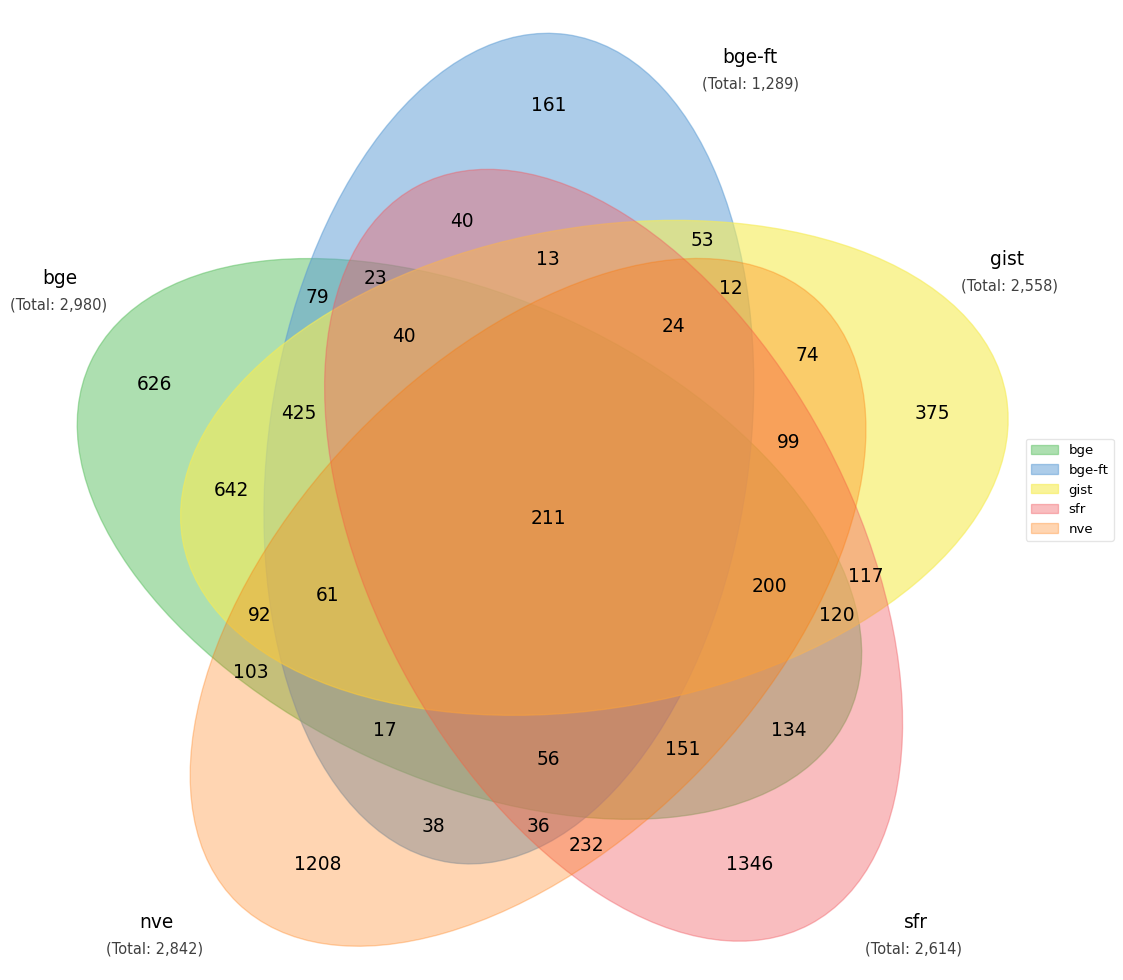
\includegraphics[width=0.8\textwidth]{venn_with_totals_evaldata.png}
\caption[Venn Diagram of Misclassified Pairs]{Venn diagram illustrating the overlap of misclassified pairs on the test dataset between all five embedding models. The central intersection shows 211 pairs were misclassified by all models, indicating shared data challenges.}
\label{fig:venn_misclassified}
\end{figure}
\begin{figure}[tb]
    \captionsetup{skip=5pt}
\centering
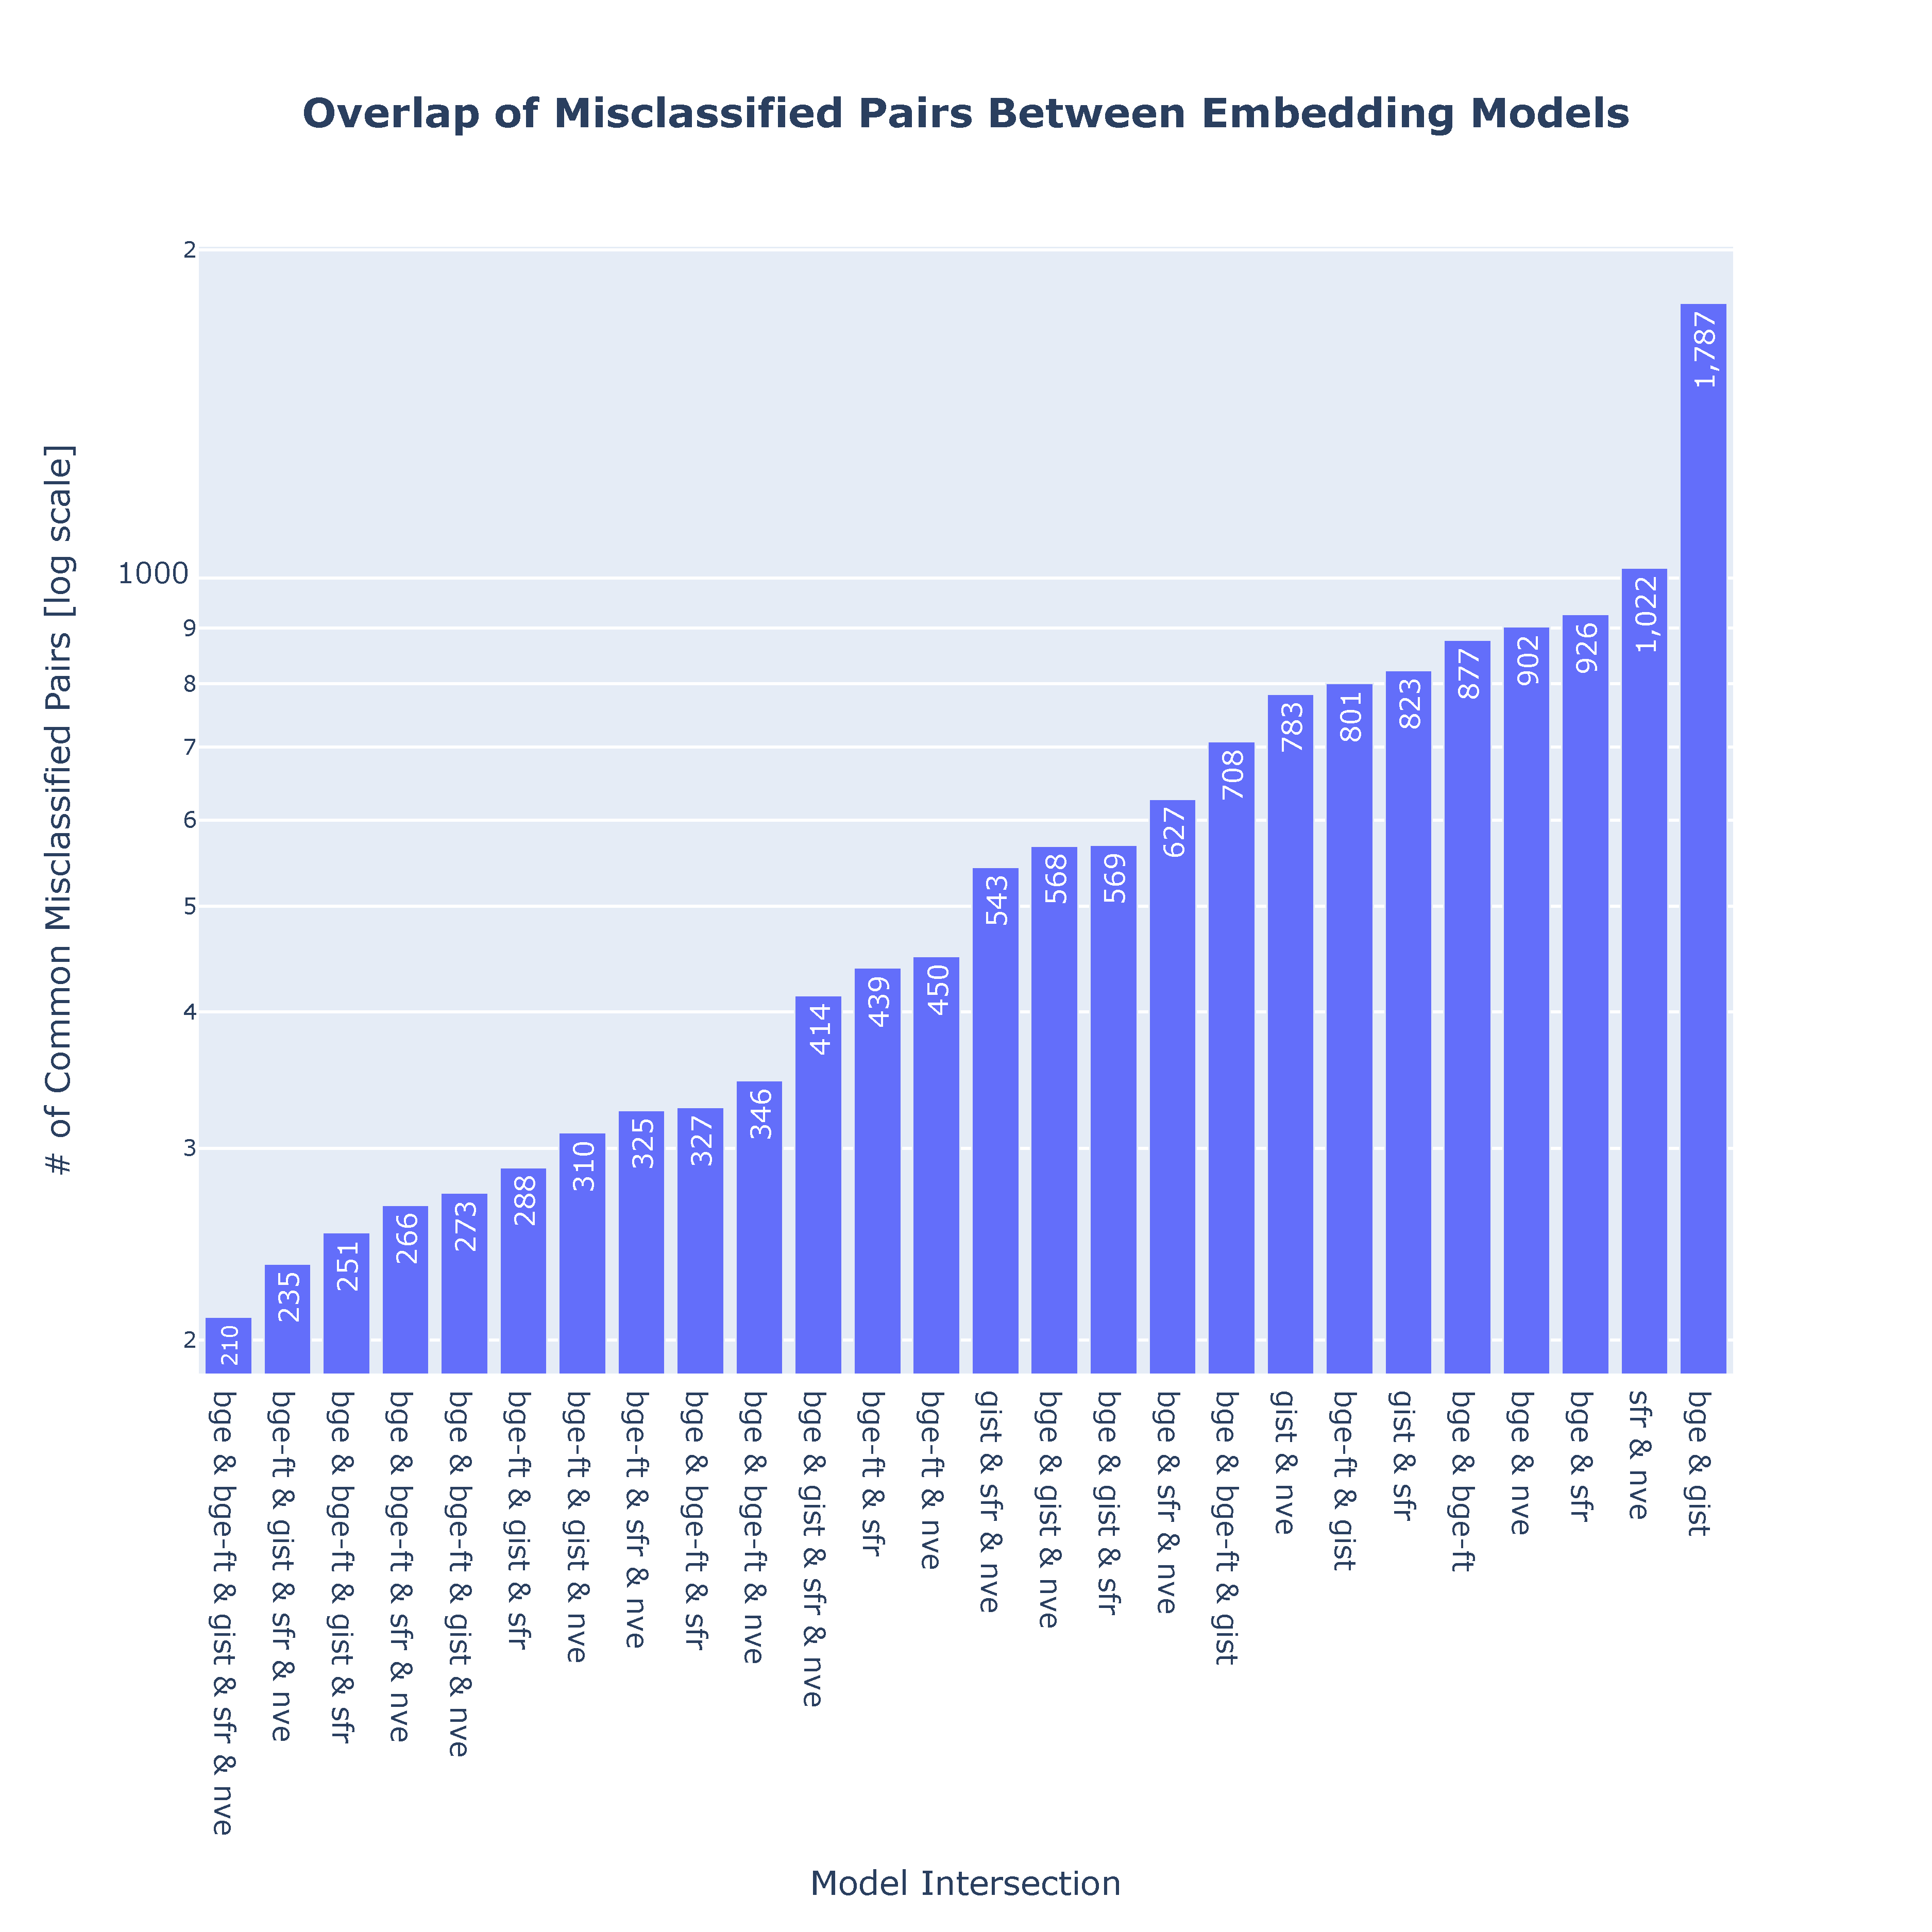
\includegraphics[width=0.8\textwidth,trim={15mm 5mm 65mm 78mm},clip]{intersection_barchart_eval.pdf}
\caption[Model Overlap for Misclassified Pairs]{Number of common misclassified pairs between all model combinations on the test dataset. The high counts of common errors across different models point to similar challenges inherent in the data.}
\label{fig:intersection_barchart}
\end{figure}

\subsection{Qualitative Analysis of False Positives}\label{ch:4.6.2}
A False Positive (FP) occurs when two non-equivalent courses are incorrectly classified as equivalent. This type of error carries meaningful real-world consequences, as it could lead a student to waste time and tuition on a non-transferable course. The analysis identified two primary causes:
\begin{itemize}
    \item \textbf{Topical Overlap without True Equivalence:} This error arises when courses cover the same broad subject but differ in scope such as academic level or their position in a curricular sequence. The model correctly identifies high semantic similarity but fails to capture the nuanced distinctions that make the courses non-equivalent. An example is the pair of PHYS-4D and PHYS-4A from Foothill College, which are sequential calculus-based physics courses covering modern and classical mechanics, respectively. Their shared title and subject matter create high semantic overlap, but they are not equivalent for transfer purposes (Appendix~\ref{app:topicoverlap}).
    \item \textbf{Ambiguous or Vague Course Descriptions:} This occurs when descriptions are too brief or use generic language, lacking the specific detail needed for differentiation. This is a known challenge in the field of short-text semantic similarity, where a lack of rich context inherently increases ambiguity~\cite{app13063911}. For example, the description for COMM-1 at Saddleback College uses abstract language like ``processes of communication'' and ``development of ideas,'' which could be semantically close to a wide range of introductory courses in public speaking, rhetoric, or even philosophy (Appendix~\ref{app:fpvague}).
\end{itemize}

\subsection{Qualitative Analysis of False Negatives}\label{ch:4.6.3}
A False Negative (FN) occurs when the system fails to identify a true equivalence, representing a missed opportunity that could cause a student to unnecessarily retake a course. These errors are predominantly a consequence of inconsistencies and information gaps in the source data itself:
\begin{itemize}
    \item \textbf{Semantic Divergence in Descriptions:} This error occurs when two officially equivalent courses are described using vastly different terminology, phrasing, or pedagogical focus. For example, a pair of courses with the same C-ID (CDEV-100) are described differently: one (Bakersfield College's CHDV-B21) uses the language of traditional developmental psychology (``psychosocial'', ``milestones''), while the other (Cerritos College's CD-110) uses the language of social justice pedagogy (``diversity and inclusion,'' ``anti-bias curriculum''). The model correctly assesses the texts as semantically dissimilar; the failure lies in the inconsistency of the source data, where the ground truth asserts an equivalence not present in the text (Appendix~\ref{app:semdiv}).
    \item \textbf{Incomplete or Minimalist Descriptions:} This error arises when one or both course descriptions in an equivalent pair are too sparse to provide sufficient textual signal for the model to establish a confident match. An example is a pair of Physics courses (both C-ID PHYS-205), where one description from Moorpark College is rich with keywords like ``kinematics'' and ``Newtonian mechanics,'' while the corresponding description from Imperial Valley College is a brief, high-level survey summary, lacking the conceptual depth for the model to map the two courses closely (Appendix~\ref{app:fnvague}).
    \item \textbf{Data Quality and Labeling Errors:} In some cases, a false negative can be traced back to a fundamental error in the ground-truth data. A striking example is a pair of courses labeled with C-ID SOCI-125, where the description for one course is for an LGBTQ+ studies class, while the description for the other is for an introduction to statistics. This is almost certainly a data entry error in the source corpus. The model correctly identifies the courses as non-equivalent but is penalized with a false negative because the ground-truth label is erroneous (Appendix~\ref{app:labelerror}).
\end{itemize}

\section{Summary}\label{ch:4.7}
This chapter presented a comprehensive, multi-stage empirical evaluation that validated the proposed decoupled, deep metric learning framework. The investigation began by establishing a performance baseline using a direct Large Language Model approach, which, while capable, highlighted considerable limitations that motivated the development of the primary pipeline. The subsequent validation of the framework's core components proved highly successful. Our ablation study confirmed that the novel composite distance vector, \(\Delta_c\), is a demonstrably superior feature representation.

The most consequential performance gain was achieved through domain-specific fine-tuning. The resulting BGE-ft model, adapted to the PPM Corpus using a \verb|BatchSemiHardTripletLoss| objective, was shown to be statistically superior to all off-the-shelf models, providing strong empirical evidence for the efficacy of applying deep metric learning to engineer a bespoke embedding space for the course catalog domain. In the final evaluation stage, while all four finalist classifiers achieved exceptionally high \(F_1\)-scores, a nuanced trade-off between peak accuracy and computational efficiency emerged. Statistical analysis identified the Support Vector Machine (SVM) as the most accurate and consistent classifier, whereas Random Forest and XGBoost proved to be significantly more efficient, making them compelling alternatives for real-world deployment.{\setlength{\emergencystretch}{5em}\par}

Finally, a qualitative misclassification analysis provided a essential perspective on the system's performance. The analysis revealed that despite the high accuracy of the optimized pipeline, the remaining errors are not random but are largely systemic, stemming from challenges inherent to the data itself, such as semantic divergence in the descriptions of equivalent courses, ambiguity from vague descriptions, and fundamental data quality errors. The comprehensive evaluation, therefore, concludes that while the proposed framework is highly effective, the primary bottleneck for further improvement likely does not lie in the model architecture or classification algorithm, but in the quality and consistency of the source data.